% Masters/Doctoral Thesis 
% LaTeX Template
% Version 2.5 (27/8/17)
%
% This template was downloaded from:
% http://www.LaTeXTemplates.com
%
% Version 2.x major modifications by:
% Vel (vel@latextemplates.com)
%
% This template is based on a template by:
% Steve Gunn (http://users.ecs.soton.ac.uk/srg/softwaretools/document/templates/)
% Sunil Patel (http://www.sunilpatel.co.uk/thesis-template/)
%
% Template license:
% CC BY-NC-SA 3.0 (http://creativecommons.org/licenses/by-nc-sa/3.0/)
%
%%%%%%%%%%%%%%%%%%%%%%%%%%%%%%%%%%%%%%%%%

 
%----------------------------------------------------------------------------------------
%	PACKAGES AND OTHER DOCUMENT CONFIGURATIONS
%----------------------------------------------------------------------------------------

\documentclass[
12pt, % The default document font size, options: 10pt, 11pt, 12pt
% oneside, % Two side (alternating margins) for binding by default, uncomment to switch to one side
english, % ngerman for German
singlespacing, % Single line spacing, alternatives: onehalfspacing or doublespacing
% draft, % Uncomment to enable draft mode (no pictures, no links, overfull hboxes indicated)
%nolistspacing, % If the document is onehalfspacing or doublespacing, uncomment this to set spacing in lists to single
liststotoc, % Uncomment to add the list of figures/tables/etc to the table of contents
% toctotoc, % Uncomment to add the main table of contents to the table of contents
% parskip, % Uncomment to add space between paragraphs
% nohyperref, % Uncomment to not load the hyperref package
headsepline, % Uncomment to get a line under the header
% chapterinoneline, % Uncomment to place the chapter title next to the number on one line
% consistentlayout, % Uncomment to change the layout of the declaration, abstract and acknowledgements pages to match the default layout
]{MastersDoctoralThesis} % The class file specifying the document structure

\usepackage[utf8]{inputenc}  % Required for inputting international characters
\usepackage[T1]{fontenc}  % Output font encoding for international characters
\usepackage{amsmath, amsfonts, amssymb}
% \usepackage[StdBrackets]{envmath}
% \usepackage{physics}
\usepackage[autostyle=true]{csquotes}  % Required to generate language-dependent quotes in the bibliography
% \usepackage{subcaption}
% \usepackage{graphicx}
\usepackage{subfig}  % needed for the tricks I do on the titlepage
\usepackage{siunitx}
\usepackage{annotate-equations}
\usepackage{tabularray}
% \usepackage{thumbs}  % add thumbs to the sides of pages
\usepackage{titlesec}  % style chapter titles
\usepackage[bibstyle=numeric, citestyle=numeric-comp, sorting=none]{biblatex}
\usepackage[colorlinks=true, allcolors=blue]{hyperref}
\usepackage[capitalise, nameinlink]{cleveref}


% \usepackage{utopia}  % Use the Palatino font
% \usepackage{newtxtext,newtxmath}  % Use the TeX Gyre Termes font
\usepackage{tgheros}  % Use the TeX Gyre Heros font

\setcounter{secnumdepth}{3}
\addbibresource{Bibliography.bib}
\renewcommand{\eqnhighlightheight}{\vphantom{\hat{H}}\mathstrut} % custom 0-width height

%----------------------------------------------------------------------------------------
%	MARGIN SETTINGS
%----------------------------------------------------------------------------------------

\geometry{
	paper=a4paper, % Change to letterpaper for US letter
	inner=2.5cm, % Inner margin
	outer=2.5cm, % Outer margin
	bindingoffset=.5cm, % Binding offset
	top=1.5cm, % Top margin
	bottom=1.5cm, % Bottom margin
	% showframe, % Uncomment to show how the type block is set on the page
}


%----------------------------------------------------------------------------------------
%	THESIS INFORMATION
%----------------------------------------------------------------------------------------

\thesistitle{Local Interaction Region Coupling Correction for the LHC} % Print with \ttitle
\supervisor{Prof. Carsten \textsc{Welsch}} % Print with \supname
\examiner{} % Print with \examname
\degree{Doctor of Philosophy} % Print with \degreename
\author{Felix \textsc{Soubelet}} % Print with \authorname
\addresses{} % Print with \addressname
\subject{Accelerator Physics} % Print with \subjectname
\keywords{} % Print with \keywordnames
\university{\href{https://www.liverpool.ac.uk/}{University of Liverpool}} % Print with \univname
\department{\href{https://www.liverpool.ac.uk/physical-sciences/}{School of Physical Sciences}} % Print with \deptname
\group{\href{https://www.liverpool.ac.uk/quasar/}{QUASAR Group}} % Print with \groupname
\faculty{\href{http://home.cern}{CERN}} % Print with \facname


%----------------------------------------------------------------------------------------
%	START OF DOCUMENT - FRONTMATTER
%----------------------------------------------------------------------------------------


\begin{document}

\frontmatter % Use roman page numbering style (i, ii, iii, iv...) for the pre-content pages

\pagestyle{plain} % Default to the plain heading style until the thesis style is called for the body content


\begin{titlepage}
\begin{center}

\vspace*{.06\textheight}
\vspace{1cm}
{\scshape\LARGE \univname\par} % University name
\vspace{0.8cm}

\begin{figure}[ht]
    \centering
    
\includegraphics[width=\textwidth]{Figures/Logos/UoLlogo.eps}
\end{figure}

\HRule \\[0.4cm] % Horizontal line
{\huge \bfseries \ttitle\par}\vspace{0.4cm} % Thesis title
\HRule \\[1cm] % Horizontal line

\vspace{1cm}

\begin{minipage}[t]{0.4\textwidth}
\begin{flushleft} \large
\text{Submitted by:}\\
\href{https://orcid.org/my-orcid?orcid=0000-0001-8012-1440}{\authorname} % Author name - remove the \href bracket to remove the link
\end{flushleft}
\end{minipage}
\begin{minipage}[t]{0.4\textwidth}
\begin{flushright} \large
\text{Supervised by:}\\
\href{https://www.researchgate.net/profile/Tobias-Persson}{Dr. Tobias~\textsc{Persson}}\\
\href{https://orcid.org/0000-0002-9857-1703}{Dr. Rogelio~\textsc{Tomás}}\\
\href{https://orcid.org/0000-0002-5410-7706}{Dr. Oznur~\textsc{Apsimon}}\\
\href{https://orcid.org/0000-0001-7085-0973}{\supname}\\
\end{flushright}
\end{minipage}

\vspace{1.5cm}

\vfill

\large {Thesis submitted in accordance with the requirements of the\\}
\univname, \deptname \\
\large {for the degree of Doctor in Philosophy}

\vfill

{\large \today}\\[4.5cm] % Date

\vfill
\end{center}
\end{titlepage}
% ----- Commands for recurrent expressions ----- %

% Command for asterisks
\newcommand{\asterisk}{\(^{\ast}\) }  % needs the trailing space


% ----- Commands for recurrent expressions in math mode ----- %

% Command for the absolute value of something
\newcommand{\abs}[1]{\left\lvert #1 \right\rvert}

% Command for the complex conjugate of something
\newcommand{\conj}[1]{#1^{\ast}}

% \dedicatory{For/Dedicated to/To my\ldots}
% \begin{abstract}

In order to further expand our knowledge of the structure of matter and the workings of our universe, scientists are constantly seeking to collide particles at ever-increasing energies and with higher \gls{luminosity}.
So is the task of the \gls{LHC} at \acrshort{CERN}, the highest energy particle accelerator and collider to date, and the goal of its future upgrade into the \gls{HL-LHC}.
This constant progress in performance requires more intense beams and smaller beam sizes at collisions points as well as a tight control of these parameters.
Thus, successful operation of large-scale particle colliders heavily depends on the precise correction of magnet field or alignment errors present in the machine.

In the \gls{LHC}, transverse \gls{betatron_coupling} has been shown to have a significant impact on both the beam dynamics and luminosity production due to uncompensated sources close to the \glspl{IP}.
However, current measurement methods are not sufficient for precise local coupling measurement at the \gls{IP}, and the impact of these sources has so far been left uncompensated.
This thesis covers work done in an effort to determine and correct Interaction Region (\acrshort{IR}) local coupling.

A key tool presented in this document is the designed \gls{RWS}, a new optics configuration which allows the determination of local coupling corrections based on correlated global variables such as the closest tune approach \glssymbol{Cminus}.
The validity of this new method has been demonstrated through simulations and experimental measurements taken during the \gls{LHC} \Gls{run}~\num{3} commissioning in~\num{2022}, where determined corrections were applied and led to a measured luminosity increase of \qty{9.7}{\percent} and \qty{3.5}{\percent} at the \acrshort{ATLAS} and \acrshort{CMS} detectors, respectively.
Additionally, the application of machine learning techniques for high complexity problems such as the detection of coupling sources in the \gls{LHC} \acrshortpl{IR} has been explored, yielding promising results but requiring some more improvements to be operationally viable.
Finally, optics studies which revealed avenues for improvements in the optics measurements done at the LHC are also presented.

\end{abstract}

\glsresetall                                     % reset glossary entries counts for the next chapter

% \begin{declaration}
\addchaptertocentry{\authorshipname} % Add the declaration to the table of contents

\vspace{1cm}

I, \authorname, declare that this thesis and the work presented in it are my own, done while in candidature for a doctorate degree.
This thesis was not used, in whole or in part, to achieve an academic degree.
No external sources were used without declaration in the text: any thoughts from others or literal quotations are clearly marked and where I have quoted from the work of others, the source is always given.
Except for such quotations, this thesis is entirely my own work.\\

Several studies and results presented in this document have already been published, and a summary of these references is given below.
The following articles report on work that was included in this thesis:
\newline \newline
\noindent\cite{IPAC:Soubelet:Prospect_IR_Coupling_Correction_LHC_Run3}: F. Soubelet \textit{et al.}, "Prospects for Local Interaction Region Coupling Correction at the LHC in Run~\num{3}", in Proceedings of \num{12}th Int. Particle Accelerator Conf. (IPAC'21), Campinas, Brazil, MOPAB007, \num{2021}.
\newline \newline
\noindent\cite{IPAC:Soubelet:First_Corrections_IR_Local_Coupling_LHC_Run3}: F. Soubelet \textit{et al.}, "First Interaction Region Local Coupling Corrections in the LHC Run~\num{3}", in Proceedings of \num{13}th Int. Particle Accelerator Conf. (IPAC'22), Bangkok, Thailand, WEPOPT007, \num{2022}.
\newline \newline
\noindent\cite{IPAC:Soubelet:Supervised_Machine_Learning_Local_Coupling_Sources_Detection_LHC}: F. Soubelet \textit{et al.}, "Supervised Machine Learning for Local Coupling Sources Detection in the LHC", in Proceedings of \num{13}th Int. Particle Accelerator Conf. (IPAC'22), Bangkok, Thailand, WEPOPT008, \num{2022}.
\newline \newline
\noindent\todo{PRAB Paper citation}: F. Soubelet \textit{et al.}, "Rigid Waist Shift: A New Method for Local Coupling Corrections in the LHC Interaction Regions", Phys. Rev. Accel. Beams \todo{some number here}, \num{2023}.
\newline \newline
\noindent\todo{IPAC23 Paper citation}: F. Soubelet \textit{et al.}, "Prospect of Operating with Limited Skew Quadrupole Corrector Availability in the LHC Interaction Regions", in Proceedings of \num{14}th Int. Particle Accelerator Conf. (IPAC'23), Venice, Italy, MOPL044, \num{2023}.
\newline
\newline
\indent
The following articles are studies that were contributed to by myself but are not included in this thesis:
\newline \newline
\noindent\cite{IPAC:Tomas:Run2_Experience_View_LHC_HLLHC}: F. Carlier \textit{et al.}, "LHC Run~\num{2} Optics Commissioning Experience in View of HL-LHC", in Proceedings of \num{10}th Int. Particle Accelerator Conf. (IPAC'19), Melbourne, Australia, MOPMP033, \num{2019}.
\newline \newline
\noindent\cite{HPC:Tracey:AI_Holistic}: R. Tracey \textit{et al.}, "AI-Driven Holistic Approach to Energy Efficient HPC", in ISC High Performance \num{2020}: High Performance Computing, pp \num{267}-\num{279}, \num{2020}.
\newline \newline
\noindent\cite{REPORT:Apollinari:HL_LHC_TDR}: I. Béjar Alonso \textit{et al.}, "High-Luminosity Large Hadron Collider (HL-LHC): Technical Design Report", in CERN Yellow Reports: Monographs, \num{2020}.
\newline \newline
\noindent\cite{IPAC:Persson:Optics_Correction_Strategy_2021}: T. Persson \textit{et al.}, "Optics Correction Strategy for Run~\num{3} of the LHC", in Proceedings of \num{12}th Int. Particle Accelerator Conf. (IPAC'21), Campinas, Brazil, WEPAB027, \num{2021}.
\newline \newline
\noindent\cite{IPAC:Maclean:Optics_Measurement_Excitation_Betatron_Oscillations_PSB}: E. Maclean \textit{et al.}, "Optics Measurement by Excitation of Betatron Oscillations in the CERN PSB", in Proceedings of \num{12}th Int. Particle Accelerator Conf. (IPAC'21), Campinas, Brazil, THPAB168, \num{2021}.
\newline \newline
\noindent\cite{IPAC:Persson:Optics_Measurements_Correction_Plans_HLLHC}: T. Persson \textit{et al.}, "Optics Measurements and Correction Plans for the HL-LHC", in Proceedings of \num{12}th Int. Particle Accelerator Conf. (IPAC'21), Campinas, Brazil, WEPAB026, \num{2021}.
\newline \newline
\noindent\cite{REPORT:OMC:Optics_Strategy_HLLHC}: X. Buffat \textit{et al.}, "Optics Measurement and Correction Strategies for HL-LHC", in CERN ATS Notes, \num{2022}. \todo{check later if this is correct}
\newline \newline
\noindent\cite{IPAC:Persson:Optics_Correction_Strategy_2022}: T. Persson \textit{et al.}, "Optics Correction Strategy for Run~\num{3} of the LHC", in Proceedings of \num{13}th Int. Particle Accelerator Conf. (IPAC'22), Bangkok, Thailand, WEPOST008, \num{2022}.
\newline \newline
\noindent\cite{IPAC:Fol:ML_Application_LHC_Optics_Commissioning}: E. Fol \textit{et al.}, "Experimental Demonstration of Machine Learning Application in LHC Optics Commissioning", in Proceedings of \num{13}th Int. Particle Accelerator Conf. (IPAC'22), Bangkok, Thailand, MOPOPT047, \num{2022}.
\newline \newline
\noindent\todo{JOSCH Paper citation}: J. Dilly \textit{et al.}, "First Operational Dodecapole Correction in the LHC", Phys. Rev. Accel. Beams \todo{paper code}, \num{2023}.
\newline \newline
\noindent\todo{IPAC23 Paper citation}: F. Carlier \textit{et al.}, "Prospect of Operating with Limited Skew Quadrupole Corrector Availability in the LHC Interaction Regions", in Proceedings of \num{14}th Int. Particle Accelerator Conf. (IPAC'23), Venice, Italy, MOPL044, \num{2023}.
\newline \newline
\noindent\cite{IPAC:Carlier:Challenges_kmodulation_LHC_Run3}: F. Carlier \textit{et al.}, "Challenges of k-Modulation Measurements in the LHC Run~3", in Proceedings of \num{14}th Int. Particle Accelerator Conf. (IPAC'23), Venice, Italy,  MOPL014, \num{2023}.
\newline \newline
\noindent\cite{IPAC:Carlier:LHC_Run3_Optics_Correction}: F. Carlier \textit{et al.}, "LHC Run~3 Optics Correction", in Proceedings of \num{14}th Int. Particle Accelerator Conf. (IPAC'23), Venice, Italy,  MOPL015, \num{2023}.
\newline \newline
\todo{Check all above and add anything else that I forgot. Also fix the bibtex for IPAC23 papers.}
\end{declaration}

\cleardoublepage
% \begin{acknowledgements}
% \addchaptertocentry{\acknowledgementname} % Add the acknowledgements to the table of contents
\vspace{0.8cm}

% Somehow, this section turned out to be the hardest to write out of this thesis.
Now that the main results of several years of work have been summarized in this little document and, as this writing comes to an end, it is time to look back and thank the many people that have contributed and supported me along the way.
\newline

First and foremost, I wish to thank Tobias Persson with all my heart for his kind supervision and unwavering support during those years.
I consider this PhD to be divided into a before and an after, and you to be the turning point.
I can never thank you enough for your patience, advice, guidance, encouragements and enthusiasm, without which I know I would not have crossed the finish line.
My heartfelt thanks go to Rogelio Tomás as well for keeping my best interest in mind, and for your continuous help and wise feedback throughout.
\newline

A few special people now need to be thanked here.
They have all, each in their own way, significantly contributed to helping me through this long journey.
\newline

A big thanks to Joschua Dilly for your enthusiasm for programming, "clean code" and scientific computing.
Thanks for the reviews, for the late night pull requests, the scientific discussions, the coffees, the control room banter and for your \LaTeX \ black magic knowledge.
This document would not have looked as good without you.

To Félix Carlier, or "Félix number \num{1}", thank you for taking the time to explain so much of the non-linear dynamics theory to me, and for providing advice on the writing of this document.
Your thesis, that you so kindly gave me a physical copy of, has been a great source of inspiration and has set a high standard of quality.

Thank you to Michael Hofer for the countless questions you have answered, for being the first to guide me through the perilous land of Resonance Driving Terms, and for being such an encyclopedia of knowledge and Indico links.

To Elena Fol, thank you for showing me how to teach the machines, for the coffee talks and for being such a little ray of sunshine every day (except when it's cold).

To Axel Poyet, thank you for being you and being there every step of the way, from close and afar.
Thanks for the friendship, the help, the jokes, the sarcasm, the shared struggle and all of the silliest moments: it has been great.

Thank you to Konstantinos Paraschou for being a great flatmate through part of this journey, and getting through the pandemic lockdowns with me: shared mental breakdowns are strangely cathartic.
As you already (don't) know, "book boom".

Thanks also go to my family for their support, patience and encouragements.
\newline

Many other people - so many, actually - have contributed one way or another to this adventure, and a few group mentions are in order.
\newline

My thanks go to all the past and current members of the OMC team for the great work environment of this group, and for their cheerful company during all these hours - mostly nights and weekends - spent in the control room.
I am equally grateful to the LHC Operations team for their collaboration, for accepting me in their midst for a short time, and in particular to Michi Hostettler for being such a source of knowledge and always eager to provide help and advice.
Similar thanks go to the wonderful folks at the IBM Hartree center for taking me in during my placement, especially Vadim Elisseev and Rob Tracey for their close supervision.

Many thanks to some special teachers who have played a bigger part than they know turning me into the scientist I am today: Mr. Bourquard for fostering my curiosity in all things physics-related, and Mr. Beck for helping me find - at my own speed - the beauty in mathematics.
Thank you to Jonathan Ferreira for the passionate and passionating plasma lectures, Alexis Nuttin for equally great neutronics classes; and Elsa Merle-Lucotte for the degree of her involvment helping students find their way.

To all the people I have walked the PhD road with - Thibault, Marie, Eva, Mathilde, Anaïs, Floriane, Guillaume, Mathieu, Nico, Elsa, Élisabeth, Diane, Pauline, Laurène, Émilien, Marouane, Luis and many more - a thousand thanks for your comradeship and the myriad of great moments we have shared.
I wish you to find success and happiness in your journey, wherever it may take you.
\newline

As a final word, a big "thank you!" to all scientists who have advanced this beautiful field of physics, have led to the design, creation and operation of the LHC, and overall have made my PhD possible.
As was put so well into words by Sir Isaac Newton: "If I have seen further, it is by standing on the shoulders of giants."

\end{acknowledgements}
% \newpage
\vspace*{0.4\textheight}
\begin{center}
	\noindent\enquote{\itshape Everything always breaks...}\bigbreak
	Tobias Hakan Bjorn Persson.
\end{center}

\tableofcontents % Prints the main table of contents
\listoffigures % Prints the list of figures
\listoftables % Prints the list of tables

% \begin{abbreviations}{ll} % Include a list of abbreviations (a table of two columns)

\textbf{ABP}        & CERN's \textbf{A}ccelerators and \textbf{B}eam \textbf{P}hysics group\\
\textbf{AD}         & \textbf{A}ntiproton \textbf{D}ecelerator\\
\textbf{ALICE}      & \textbf{A} \textbf{L}arge \textbf{I}on \textbf{C}ollider \textbf{E}xperiment\\
\textbf{ATLAS}      & \textbf{A} \textbf{T}oroidal \textbf{L}HC \textbf{A}pparatu\textbf{S}\\
\textbf{AWAKE}      & \textbf{A}dvanced \textbf{WAK}efield \textbf{E}xperiment\\
\textbf{BE}         & CERN's \textbf{BE}ams department\\
\textbf{BPM}        & \textbf{B}eam \textbf{P}osition \textbf{M}onitor\\
\textbf{CERN}       & \textbf{E}uropean \textbf{O}rganization for \textbf{N}uclear \textbf{R}esearch\\
\textbf{CMS}        & \textbf{C}ompact \textbf{M}uon \textbf{S}olenoid\\
\textbf{DA}         & \textbf{D}ynamic \textbf{A}perture\\
\textbf{ELENA}      & \textbf{E}xtra \textbf{L}ow \textbf{EN}ergy \textbf{A}ntiproton ring\\
\textbf{HERA}       & \textbf{H}adron-\textbf{E}lectron \textbf{R}ing \textbf{A}ccelerator\\
\textbf{HiRadMat}   & \textbf{H}igh \textbf{Rad}iation to \textbf{Mat}erials\\
\textbf{HL-LHC}     & \textbf{H}igh \textbf{L}uminosity \textbf{L}arge \textbf{H}adron \textbf{C}ollider\\
\textbf{HSS}        & CERN's \textbf{H}adron \textbf{S}ynchrotron \textbf{S}ingle particle effects section\\
\textbf{IP}         & \textbf{I}nteraction \textbf{P}oint\\
\textbf{IR}         & \textbf{I}nteraction \textbf{R}egion\\
\textbf{ISOLDE}     & \textbf{I}sotope \textbf{S}eparator \textbf{O}n \textbf{L}ine \textbf{DE}tector\\
\textbf{LEIR}       & \textbf{L}ow \textbf{E}nergy \textbf{I}on \textbf{R}ing\\
\textbf{LHC}        & \textbf{L}arge \textbf{H}adron \textbf{C}ollider\\
\textbf{LHCb}       & \textbf{L}arge \textbf{H}adron \textbf{C}ollider \textbf{b}eauty\\
\textbf{MAD}        & \textbf{M}ethodical \textbf{A}ccelerator \textbf{D}esign\\
\textbf{n-TOF}      & \textbf{N}eutron \textbf{T}ime \textbf{O}f \textbf{F}light\\
\textbf{OMC}        & \textbf{O}ptics \textbf{M}easurements and \textbf{C}orrections\\
\textbf{PS}         & \textbf{P}roton \textbf{S}ynchrotron\\
\textbf{PTC}        & \textbf{P}olymorphic \textbf{T}racking \textbf{C}ode\\
\textbf{RDT}        & \textbf{R}esonance \textbf{D}riving \textbf{T}erm\\
\textbf{SPS}        & \textbf{S}uper \textbf{P}roton \textbf{S}ynchrotron\\

\end{abbreviations}
% \begin{constants}{lr@{${}={}$}l} % The list of physical constants is a three column table

The \SI{}{} command is provided by the siunitx package, see its documentation for instructions on how to use it

Speed of Light & $c_{0}$ & \SI{2.99792458e8}{\meter\per\second} (exact)\\
Constant Name & $Symbol$ & $Constant Value$ with units\\

\end{constants}
% \begin{symbols}{lll} % Include a list of Symbols (a three column table)

$a$ & distance & \si{\meter} \\
$P$ & power & \si{\watt} (\si{\joule\per\second}) \\
Symbol & Name & Unit \\

\addlinespace % Gap to separate the Roman symbols from the Greek

$\omega$ & angular frequency & \si{\radian} \\

\end{symbols}


%----------------------------------------------------------------------------------------
%	THESIS CONTENT - CHAPTERS
%----------------------------------------------------------------------------------------

\mainmatter % Begin numeric (1,2,3...) page numbering

\pagestyle{thesis} % Return the page headers back to the "thesis" style

%----------------------------------------------------------------------------------------
%	REDEFINE CHAPTER TITLE STYLE
%----------------------------------------------------------------------------------------

% See doc of titlesec page 22 (https://mirror2.sandyriver.net/pub/ctan/macros/latex/contrib/titlesec/titlesec.pdf)
% TODO: fix the slight antisymmetry in vspace bellow CHAPTER N

\titleformat{\chapter}[display]
{\Large\filcenter}
{\titlerule[1pt]%
\vspace{1pt}%
\titlerule
\vspace{1pc}%
\LARGE\MakeUppercase{\chaptertitlename} \thechapter}{1pc}
{\titlerule
\vspace{1pt}%
\titlerule[1pt]%
\vspace{1pc}%
\Huge}
\chapter{Introduction}
\label{chapter:introduction}

\begin{noteblock}
    In this document a distinction is made between glossary items and acronyms, and locally relevant terms and concepts.
    The former will appear in \textcolor{cern}{blue} and are clickable links bringing the reader back to the glossary such as the following: \gls{optics}.
    The latter will appear in \concept{orange} and are an indication of a term or concept that is important to the content at hand but does not necessarily warrant its own entry in the glossary.
\end{noteblock}

\section{Motivations}

Accelerator physics as a branch of physics has its roots nearly a century ago with the pioneering work of E.~Lawrence~\cite{PR:Lawrence:Production_High_Speed_Light_Ions} inventing the cyclotron, and shortly after in \num{1932} when J.~Cockcroft and E.~Walton~\cite{LLC:Cockcroft:Disintegration_Lithium_Swift_Protons,TRS:Cockcroft:Experiments_High_Velocity_Positive_Ions_1,TRS:Cockcroft:Experiments_High_Velocity_Positive_Ions_2} built the first particle accelerator that could produce nuclear reactions.
Since then accelerator physics has grown into a mature field of research with applications ranging from cancer treatment and the production of medical isotopes to material science such as the analysis of archeological items, but also many industrial uses.

However, \gls{HEP} - the study of the fundamental constituents of matter - has historically been the main drive to push the boundaries of accelerator science.
Respectively, one of the most significant contributions of this field has been the design, construction and operation of particle colliders providing data for experiments at the forefront of \gls{HEP} research, such as the \gls{LHC} at \acrshort{CERN}, the highest energy and most technologically advanced particle accelerator yet built.
These contributions recently culminated with the discovery of the Higgs boson by the \acrshort{ATLAS} and \acrshort{CMS} experiments at the \acrshort{LHC} in \num{2012}~\cite{PLB:ATLAS:Observation_Higgs_Boson, PLB:CMS:Observation_Higgs_Boson}, which Peter Higgs and François Englert were awarded the \num{2013} Nobel Prize in Physics for theorizing nearly \num{50} years prior~\cite{PRL:Higgs:Broken_Symmetries_Masses_Gauge_Bosons,PRL:Englert:Broken_Symmetry_Mass_Gauge_Vector_Mesons}.

Since then experiments at the \gls{LHC} keep analyzing data from collisions to probe in more details the now uncovered mechanisms, as well as attempt to discover physics beyond the Standard Model such as supersymmetry or dark matter.
To this end, the LHC has kept pushing its performance to even higher energies and \gls{luminosity}.
The machine has already undergone two \glspl{longshutdown} during which it was upgraded, and is currently in the \Gls{run}~\num{3} of its operation.
Another shutdown is planed a few years from now to upgrade the accelerator to the \gls{HL-LHC}~\cite{Website:HLLHC}, which aims to increase the \gls{luminosity} of the collider by a factor of \num{10}.

Increasing the luminosity of the machine however is not without its challenges and limitations, and in order to achieve an optimal performance an understanding and control of the dynamics of the particle beams is essential.
One such limitation to the delivery of optimal \gls{luminosity} is the so-called local linear \gls{betatron_coupling} in the \glspl{IR}, which can lead to a significant decrease in collision numbers if left uncorrected.

The focus of this thesis is on the handling of local linear coupling in the \glspl{IR} of the \gls{LHC}, and the development of a new method to measure and correct the phenomenon, improving the performance of the accelerator.
By addressing this issue, the research presented in this document aims to contribute to the ongoing efforts to push the performance of the \gls{LHC} to even greater heights, and to hopefully enable new discoveries in the field of particle physics.

\section{Thesis Outline}

This document exposes work done on the matter of local linear coupling correction in the LHC, and of this thesis at large.
Across studies a focus is kept on the main \glspl{IR} of the \gls{LHC}, \numlist{1;5}, which are more error-sensitive due to their optics configurations.

As a first step and to allow the reader to follow the details of this work, \cref{chapter:theory} gives a detailed introduction to the world of accelerator physics and beam dynamics.
The chapter starts with the linear beam dynamics as the core foundation to any particle accelerator, then carries on with non-linear phenomenology present in more complex machines in order to introduce necessary concepts and quantities of interest to the work presented in this document, such as \glspl{RDT}.
A section is dedicated to \gls{betatron_coupling} and its parametrization, and another to \gls{luminosity} as a key performance indicator of a collider.

Also in view of helping the reader follows \cref{chapter:lhc_omc} which opens on a comprehensive overview of the \gls{LHC} machine and its operation in \Gls{run}~\num{3}, with particular attention given to the main \glspl{IR}.
The second half of the chapter offers a dive into the practice of \gls{OMC} as done at the \gls{LHC} by the \gls{OMC} team.
Insight is given on each step, going from data acquisition methods and devices to the reconstruction of quantities of interest and the determination of adjustments that would bring the machine closer to its nominal state.

The main body of work for this thesis, which offers a new experimental setup and correction method for local linear coupling in the \gls{LHC} \glspl{IR}, is detailed in \cref{chapter:ir_local_coupling}.
The chapter opens by providing the reader with a justification of the need for local linear coupling correction both for the \gls{LHC} and the future \gls{HL-LHC} machine.
An overview of the local coupling situation in the \gls{LHC} is given, including current correction methods and their limitations which stem from the specific conditions of the \gls{LHC} \glspl{IR}.
The theoretical basis for the new correction method is laid out, which relies on the leakage of \glspl{RDT} from the \glspl{IR} to the rest of the machine, and the various experimental setup tools that were developed are thoroughly presented.
Experimental measurements and data analysis from the method's application in the \gls{LHC} \num{2022} commissioning are presented as well as the resulting \gls{luminosity} improvements observed from the application of the determined corrections.
A short section is dedicated to the relevance of this method for other existing or future colliders.
Finally, the chapter offers an assessment of the realistic eventuality of one or more failure of the dedicated magnets used for coupling correction and the explored solutions.

In line with the themes of the \gls{LIV.DAT}~\cite{Website:LIVDAT} a machine learning based approach to the subject of local linear coupling has been explored, that is presented in \cref{chapter:ml_local_coupling}, which starts with a minimal overview of the relevant machine learning concepts.
The new approach to local linear coupling is presented with a focus on the data preparation, model training and achieved results.
A discussion on the potential of this machine learning approach is held, as well as the challenges to overcome to make it fully viable in \gls{LHC} operations.

Some additional work performed during this thesis is presented in \cref{chapter:others_and_software}.
While not relating directly to the main subject of this thesis, the work presented in this chapter is nonetheless relevant to either the \gls{LHC} and its operation or to the \gls{OMC} team's activities at large.

Finally, \cref{chapter:conclusion} restates the main results and conclusions from the work done in this thesis.
A discussion is held on the findings and any missing element to this work, as well as the potential avenues for future developments.
The chapter closes with a look at the future of LHC operations and potential implications of this work to other colliders.

Some additional material is provided in the appendices of this document.
\Cref{appendix:hamiltonian_derivation} offers a detailed derivation for the Hamiltonian thin kick expansion which would have been too cumbersome to include in \cref{chapter:theory}.
\Cref{appendix:naming_conventions} provides complementary, illustrated supporting material regarding the naming conventions in use for the \gls{LHC}, which the reader might find useful considering the inevitable amount of machine specific jargon used in this document.
In the spirit of completeness, \cref{appendix:experimental_knobs,appendix:inconclusive_measurements,appendix:measurement_fills} provide details on the experimental campaign relating to the studies in this thesis.
The former lists the different experimental knobs used for measurements in the LHC for the results shown in \cref{chapter:ir_local_coupling}, and the latter provides a comprehensive list of the LHC fills used for measurements.
\Cref{appendix:inconclusive_measurements} provides details on additional measurements not presented in detail in \cref{chapter:ir_local_coupling}.
Finally, \cref{appendix:code_developments} succinctly presents the main software development contributions done over the course of this PhD.

\glsresetall                                     % reset glossary entries counts for the next chapter

% Chapter 1

\chapter{Theory of Single-Particle Beam Dynamics in the Large Hadron Collider} % Main chapter title

\label{Chapter1} % For referencing the chapter elsewhere, use \ref{Chapter1}

%----------------------------------------------------------------------------------------

Beam dynamics is a field of accelerator science which is significant for the design, operation, performance, and protection of an accelerator. 
In this section an overview is given of the theories of beam dynamics which are relevant to the material presented in this thesis.
The chapter begins with a description of the linear dynamics, then progresses to deal with aspects of the non-linear dynamics, concluding with a discussion of the luminosity.

%----------------------------------------------------------------------------------------

\section{Linear Beam Dynamics}

Define concept: bend and focus particles to have them remain within the aperture tolerance of the machine.
Bend with dipoles, focus with quadrupoles typically.
% Within the linear approximation, non-linear magnetic fields are ignored and the beam dynamics is described by linear differential equations.
Figure \ref{fig:frenet_system} illustrates the Frenet-Serret coordinate system traditionally used in linear beam dynamics.
\bigbreak

\begin{figure}[!htb]
    \begin{center}
    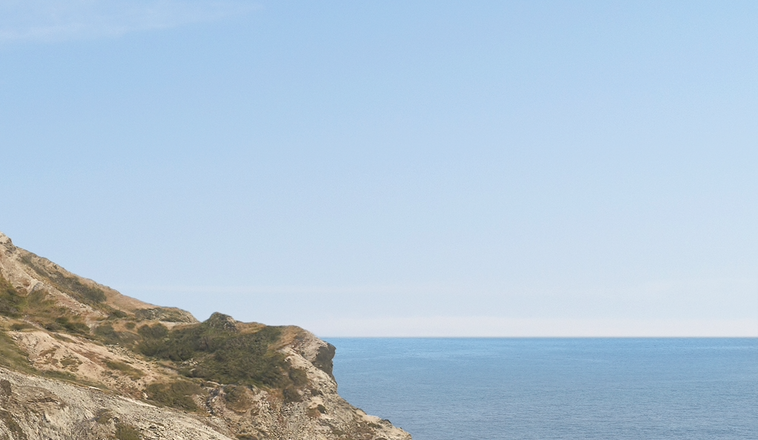
\includegraphics[width = 0.7\linewidth]{Figures/placeholder.png}
    \caption{Coordinate system for linear accelerator optics.}
    \label{fig:frenet_system}
    \end{center}
\end{figure}

Coordinate system travels longitudinally with the particle, along a reference trajectory defined by an "ideal" / "reference" / "synchronous" particle.
Define $s$ as longitudinal / curvilinear coordinate.
Define $\rho(s)$ local radius of curvature (depends on $\mathbf{B}$ and varies along ring).
Define $(x, x\prime, y, y\prime)$, coordinates of transverse phase space:
$x$ and $y$ are particle coordinates in the transverse planes (transverse displacement).
$x^{'}$ and $y^{'}$ are "divergent angles" (says Ewen) in the $x$ and $y$ plane (differentiation with respect to $s$).
\bigbreak

In linear regime, dipoles define ideal orbit for particle of \emph{reference momentum} $p_0$.
Ideal orbit goes through magnetic center of all elements and comes back on itself after a revolution, and is called a \emph{closed orbit}.
In practice dipolar errors (and more) will distort the real closed orbit from the ideal designed orbit.
Particles within the beam are distributed in amplitude (the beam occupies a finite area in $(x, x\prime, y, y\prime)$ phase space). 
The closed orbit defines the path of a particle with zero amplitude within the beam.
In practice particles oscillate around the closed orbit because of the focusing forces. 
In the LHC this focusing is provided predominantly by quadrupole magnets.
\bigbreak

From Ewen: quadrupolar fields acting on charged particles displaced from the central axis provide a restoring (focusing) force proportional to the displacement in one transverse plane, while simultaneously providing a divergent (defocusing) force in the other. 
Tradition: a quadrupole focusing in the horizontal plane and defocusing in the vertical is referred to as a \emph{focusing quadrupole}. 
A quadrupole defocusing in the horizontal plane but focusing in the vertical is referred to as a \emph{defocusing quadrupole}.
An alternating arrangement of focusing and defocusing quadrupoles, referred to as a $\mathrm{FODO}$ lattice, can create a net focusing in both planes [ref 18 ewen]. 
Figure \ref{fig:dipole_quadrupole_fields} illustrates magnetic fields in an idealized dipole and quadrupole, together with the forces exerted on a positively charged particle travelling into the page.
\bigbreak

\begin{figure}[!htb]
    \begin{center}
    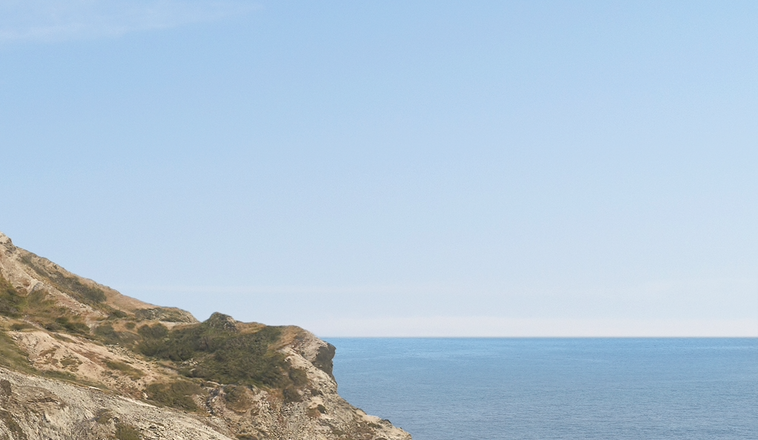
\includegraphics[width = 0.9\linewidth]{Figures/placeholder.png}
    \caption{Magnetic fields and forces in an idealized dipole (having a $cos(\phi)$ current distribution in the circular coil) and an idealized focusing quadrupole (having a $cos(2\phi)$ current distribution in the circular coil). Current in the dipole and quadrupole coils are indicated in colour. Forces exerted by the magnet on a positive charge travelling into the page are illustrated. Adapted from [19].}
    \label{fig:dipole_quadrupole_fields}
    \end{center}
\end{figure}

In circular machine focusing from quads is periodic in $s$ with a period of max the circumference of the machine.
Motion in the transverse plane is described by Hill’s equation, Eq.(\ref{eq:hill_equation}), where $k(s)$ is a periodic coefficient describing the restoring force due to the distribution of focusing fields around the ring.
\bigbreak

\begin{equation}
    u^{\prime \prime} \pm k(s) u = 0; \quad u = x, y; \quad u^{\prime} = \frac{\mathrm{d}u}{\mathrm{d}s}
    \label{eq:hill_equation}
\end{equation}
\bigbreak

Solutions to Hill’s equation take the form of Eq.(\ref{eq:hill_solution}),
\bigbreak

\begin{equation}
    \begin{aligned}
    x &= \sqrt{\beta_{x}(s) \epsilon_{x}} \cos \left(\phi_{x}(s) + \phi_{x_0}\right) \\
    y &= \sqrt{\beta_{y}(s) \epsilon_{y}} \cos \left(\phi_{y}(s) + \phi_{y_0}\right)
    \end{aligned}
    \label{eq:hill_solution}
\end{equation}

where $\epsilon$ is the emittance of a particle and is a constant of the motion at a given energy.
$\beta(s)$ is called the \emph{beta-function} and describes the variation of the oscillation envelope around the ring. 
In particle colliders such as the LHC, it is usual to denote the beta-functions at the Interaction Points (where the beams are made to collide) as $\beta^{*}$.
\bigbreak

Particle oscillate around ring, \emph{betatron oscillations}, and the number of oscillations around the ring is the \emph{tune}, $Q_{x,y}$.
The tune is defined in Eq.(\ref{eq:tune_definition}), where $\Delta \phi_{x, y}$ is the total betatron phase advance undergone by a particle during one revolution around the accelerator ring.
\bigbreak

\begin{equation}
    Q_{x, y} = \frac{1}{2 \pi} \Delta \phi_{x, y} = \frac{1}{2 \pi} \oint \frac{\mathrm{d}s}{\beta_{x, y}(s)}
    \label{eq:tune_definition}
\end{equation}

Figure \ref{fig:particle_trajectories} shows a tracking simulation of a particle undergoing such betatron oscillations in the LHC Arc12.
Dipole errors were added which have distorted the closed orbit away from the ideal path.
\bigbreak

\begin{figure}[!htb]
    \begin{center}
    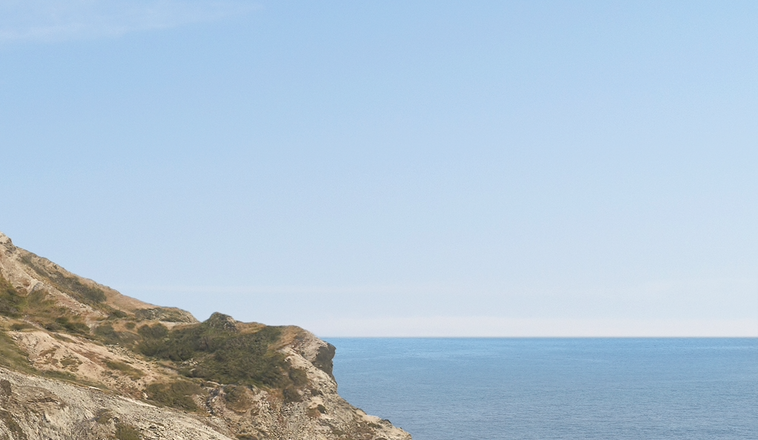
\includegraphics[width = 0.7\linewidth]{Figures/placeholder.png}
    \caption{Tracking simulation in LHC Arc12 of a particle undergoing betatron oscillations.}
    \label{fig:particle_trajectories}
    \end{center}
\end{figure}

Define the \emph{gamma-function} $\gamma(s)$ which describes the envelope of oscillations in $x\prime$ and $y\prime$.
Both are related by the \emph{alpha-function}:
\bigbreak

\begin{equation}
    \alpha_{x, y} = -\frac{1}{2} \frac{\mathrm{d}}{\mathrm{d}s} \beta_{x, y}(s) = \sqrt{\gamma_{x, y}(s) \beta_{x, y}(s) - 1}
    \label{eq:alpha_function}
\end{equation}
\bigbreak

In linear regime, trajectories are ellipses in phase space $(x, x\prime, y, y\prime)$.
$\alpha(s)$, $\beta(s)$, $\gamma(s)$ and $\epsilon$ define the equation of the ellipse, Eq.(\ref{eq:ellipse_equation}).
Figure \ref{fig:phase_space_ellipse} shows a schematic illustration of the phase space ellipse.
\bigbreak

\begin{equation}
    \gamma_{u}(s) u^{2} + 2 \alpha_{u}(s) u u^{\prime} + \beta_{u}(s) z^{\prime 2} = \epsilon \quad \text { where } u = x, y
    \label{eq:ellipse_equation}
\end{equation}
\bigbreak

\begin{figure}[!htb]
    \begin{center}
    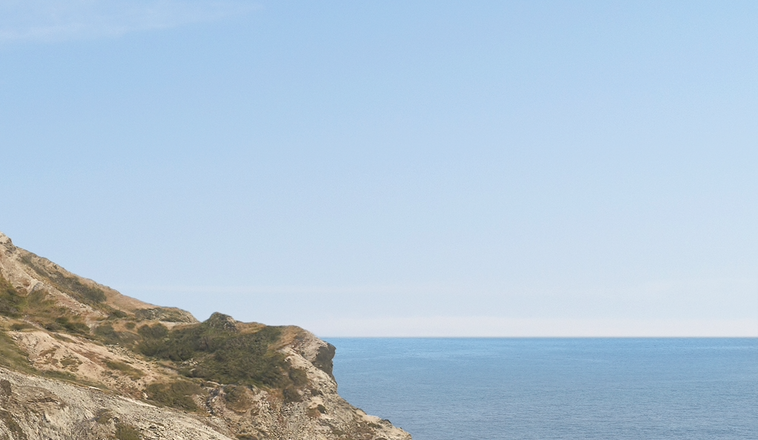
\includegraphics[width = 0.85\linewidth]{Figures/placeholder.png}
    \caption{Phase space ellipse in the transverse $z$, $z\prime$ plane, where $z$ represents either $x$ or $y$.}
    \label{fig:phase_space_ellipse}
    \end{center}
\end{figure}

Say emittance ($\epsilon$) defines phase space ellipse area.
Liouville's theorem: phase space volume (ellipse area) is constant in a closed system.
In the LHC, protons, little synchrotron radiation [ref 20 ewen] we can consider emittance a constant (but at multi-$\mathrm{TeV}$ energy radiation emission may become non-negligible).
Acceleration -> no more Liouville and \emph{physical emittance} ($\epsilon$) will reduce with increasing energy.
One can construct \emph{normalized emittance} ($\epsilon_{\gamma}$) which is invariant with beam energy.
See Eq.(\ref{eq:normalized_emittance}), where $\beta_{rel}$ and $\gamma_{rel}$ are the relativistic beta and gamma functions:
\bigbreak

\begin{equation}
    \epsilon_{\gamma} = (\beta_{\mathrm{rel}} \gamma_{\mathrm{rel}}) \epsilon
    \label{eq:normalized_emittance}
\end{equation}
\bigbreak

For a specific particle we use \emph{single particle emittance}.
Different particles may have different ones.
They will go through (undergo?) betatron oscillations of different amplitudes.
We can define \emph{beam emittance}: typically defined as the emittance corresponding $1\sigma$ amplitude in assumed Gaussian particle distribution.
\bigbreak

The phase space trajectory of a particle depends on $\alpha(s)$, $\beta(s)$, and $\gamma(s)$.
The transformation to \emph{Courant-Snyder coordinates} [ref 21 ewen] (sometimes called \emph{normalized Courant-Snyder coordinates}) removes this dependency, see Eq.(\ref{eq:courant_snyder_coordinates}),
\bigbreak

\begin{equation}
    \left(\begin{array}{c}
    \hat{u} \\
    \hat{u}^{\prime}
    \end{array}\right) = \left(\begin{array}{cc}
    \frac{1}{\sqrt{\beta_{u}(s)}} & \frac{\alpha_{u}(s)}{\sqrt{\beta_{u}(s)}} \\
    0 & \sqrt{\beta_{u}(s)}
    \end{array}\right)\left(\begin{array}{c}
    u \\
    u^{\prime}
    \end{array}\right) \quad \text{ where } u = x, y
    \label{eq:courant_snyder_coordinates}
\end{equation}

where the Courant-Snyder coordinates are denoted by \^{}.
In this new system particles follow circular trajectories in phase space.
\bigbreak

Say particles within the beam have a distribution in momentum, around designed momentum $p_0$.
For a particle that doesn't have $p_0$ we define the \textit{relative momentum deviation} $\delta$, Eq.(\ref{eq:momentum_deviation}):
\bigbreak

\begin{equation}
    \delta = \frac{p - p_0}{p_0}
    \label{eq:momentum_deviation}
\end{equation}
\bigbreak

Define \textit{magnetic rigidity}: relates magnetic flux $\mathbf{B}$ (perpendicular to motion) with local radius of curvature and particle momentum $\mathbf{P}$.
See Eq.(\ref{eq:beam_rigidity}):
\bigbreak

\begin{equation}
    \lvert \mathbf{B} \rho \rvert = \frac{\lvert \mathbf{P} \lvert}{e}
    \label{eq:beam_rigidity}
\end{equation}
\bigbreak

Say difference to $p_0$ introduce \emph{chromatic} errors into the beam dynamics.
The most important one is \emph{dispersion}.
Different momenta(um?) -> different beam rigidity -> different local radius of curvature in dipoles -> different orbit.

Deviation to reference orbit is defined by the \emph{Dispersion function}, $D(s)$ [ref 23 ewen].
In a region of non-zero dispersion the contribution to the orbit of a particle is described by Eq.(\ref{eq:dispersion_contribution_to_orbit}):
\bigbreak

\begin{equation}
    \begin{aligned}
    \Delta x_{\mathrm{dispersion}} &= D_{x}(s) \delta \\
    \Delta y_{\mathrm{dispersion}} &= D_{y}(s) \delta
    \end{aligned}
    \label{eq:dispersion_contribution_to_orbit}
\end{equation}
\bigbreak

The orbit of any given particle is defined by Eq.(\ref{eq:_particle_orbit}):
\bigbreak

\begin{equation}
    u = u_{\mathrm{betatronic}} + u_{\mathrm{dispersion}} + \left.u_{\mathrm{closed \ orbit}} \right|_{\delta = 0}
    \label{eq:_particle_orbit}
\end{equation}

%----------------------------------------------------------------------------------------

\section{Non-Linear Magnetic Multipoles}

%----------------------------------------------------------------------------------------

\section{Formalism of Non-Linear Beam Dynamics}

%----------------------------------------------------------------------------------------

\section{Phenomenology of Non-Linear Beam Dynamics}

\subsection{Chromaticity}

\subsection{Detuning with Amplitude}

\subsection{Decoherence}

\subsection{Resonances and RDTs / CRDTs}

%----------------------------------------------------------------------------------------

\section{Linear Betatron Coupling}

%----------------------------------------------------------------------------------------

\section{Luminosity}

%----------------------------------------------------------------------------------------
\chapter{Relevant Theory of Beam Dynamics for the Large Hadron Collider} % Main chapter title

\label{Chapter:Theory} % For referencing the chapter elsewhere, use \cref{Chapter:Theory}

%----------------------------------------------------------------------------------------

The design, operation, performance, and safety of a particle accelerator depend on the study of beam dynamics, a field of accelerator science.
This section provides an overview of the beam dynamics theories relevant to the material in this thesis, and more specifically beam optics.
Most of the material in this section can be found in the literature such as \cite{BOOK:Wilson:Introcution_Particle_Accelerators, BOOK:Lee:Accelerator_physics, BOOK:Minty:Measurements_Control_Charged_Particle_Beams,BOOK:Wolski:Beam_dynamics,BOOK:Chao:Handbook_Accelerator_Physics_Engineering, BOOK:Chao:Collective_instabilities}.
When not in these works, explicit references to content are given.
\todo{The chapter starts out with a description of linear dynamics, then moves on to aspects of non-linear dynamics, and ends with a discussion of luminosity}.

%----------------------------------------------------------------------------------------

\section{Linear Beam Dynamics}

The linear dynamics of an accelerator are, mainly, the endeavor to bend and focus particle beams to confine them within the machine's aperture.
To force the beam's particles into a closed trajectory, they are subjected to magnetic fields that deflect their trajectories.
The force exerted onto the beam is the Lorentz force \(F_{L}\), given by the equation:

\begin{equation}
    \vec{F_L} = \dfrac{d\vec{p}}{dt} = q (\vec{E} + \vec{v} \times \vec{B}) ,
    \label{equation:lorentz_force}
\end{equation}
where \(p\) is the particle momentum, \(q\) the particle charge, \(\vec{E}\) the electric field, \(\vec{v}\) the particle velocity and \(\vec{B}\) the magnetic field.
In most accelerators, including the LHC, the particles' speed is close to the celerity of light \(c\) and the force from the magnetic field is significantly stronger than that produced by the electric field for realistic values of \(\vec{E}\) and \(\vec{B}\).
As a result, in high energy particle accelerators magnetic fields are typically used to guide particles.
The guiding magnetic field can be expanded into a series of multipolar fields, for instance here in the horizontal plane:
% ---------- Equation ----------
\begin{align}
    B_{y} = 
    \tikz[baseline]{
        \node[draw=red,rounded corners,anchor=base] (m1)
        {$\displaystyle B_{y0}$};
        \node[below of=m1] (l1) {dipole};
        \draw[-,red] (l1) -- (m1);
    }
    +
    \tikz[baseline]{
        \node[draw=red,rounded corners,anchor=base] (m2)
        {$\displaystyle \frac{dB_{y}}{dx} x$};
        \node[below of=m2] (l2) {quadrupole};
        \draw[-,red] (l2) -- (m2);
    }
    +
    \tikz[baseline]{
        \node[draw=red,rounded corners,anchor=base] (m3)
        {$\displaystyle \frac{1}{2!} \frac{d^2B_{y}}{dx^2} x^2$};
        \node[below of=m3] (l2) {sextupole};
        \draw[-,red] (l2) -- (m3);
    }
    +
    \tikz[baseline]{
        \node[draw=red,rounded corners,anchor=base] (m4)
        {$\displaystyle \frac{1}{3!} \frac{d^3B_{y}}{dx^3} x^3$};
        \node[below of=m4] (l2) {octupole};
        \draw[-,red] (l2) -- (m4);
    }
    + \ldots
    \label{equation:magnetic_field_expansion}
\end{align}

Bending forces are supplied by dipole magnets with a magnetic field perpendicular to the beam trajectory, while focusing is typically performed with the use of quadrupole magnets.
Higher orders belong to the nonlinear dynamics and will be discussed later on.
\Cref{figure:frenet_serret_system} illustrates the Frenet-Serret coordinate system traditionally used in linear beam dynamics.

\begin{figure}[!htb]
    \begin{center}
    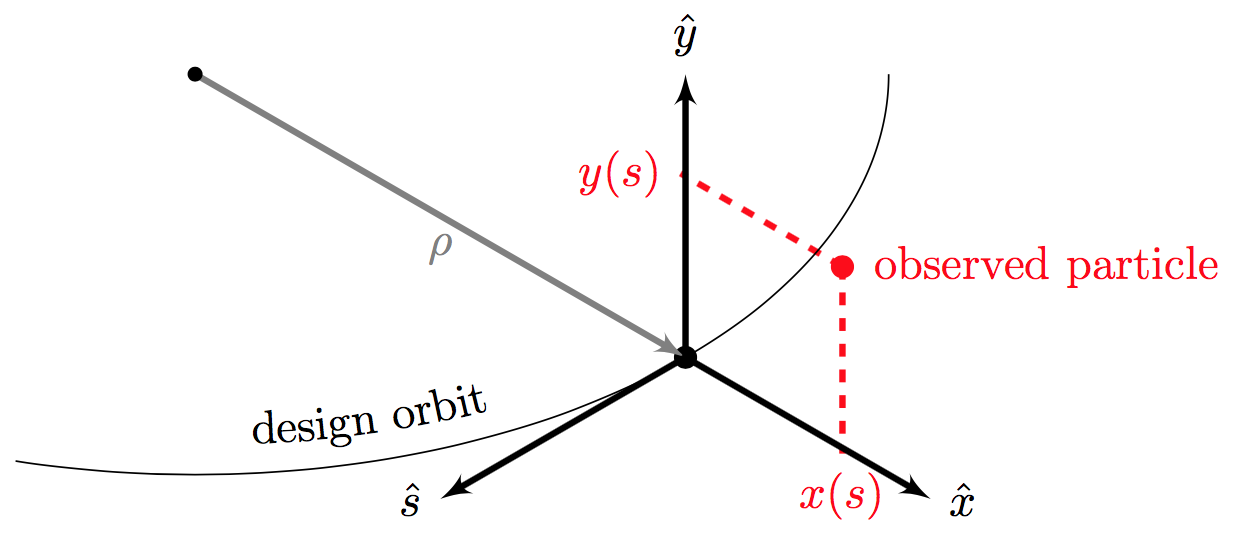
\includegraphics[width = 0.8\linewidth]{Figures/Chapter2/Frenet_Serret_Coordinate_System.png}
    \caption{The Frenet-Serret coordinate system used in accelerator physics. Here \(\hat{x}\), \(\hat{y}\), and \(\hat{s}\) form the right-handed orthogonal basis, while \(\rho\) is the local bending radius.}
    \label{figure:frenet_serret_system}
    \end{center}
\end{figure}

The coordinate system travels longitudinally with the particle, along a reference trajectory defined by an ideal, or \emph{synchronous}, particle.
The longitudinal curvilinear coordinate is \(s\), and denotes the position of the particle along the ideal orbit with respect to an arbitrary initial point at \(s = 0\).
One can define a local radius of curvature, \(\rho(s)\), which depends on the local magnetic field \(\vec{B}\) and varies along ring.
The transverse phase space is defined by \((x, x^{\prime}, y, y^{\prime})\), where \(x\) and \(y\) are a particle's coordinates in the transverse plane relative to the reference trajectory.
The \(x^{\prime}\) and \(y^{\prime}\) coordinates are \emph{divergent angles}, with the prime indicating differentiation with respect to \(s\).
\break

In the linear regime, magnetic dipoles define ideal orbit for a particle of \emph{reference momentum} \(p_0\).
This ideal orbit goes through the magnetic center of all elements in the machine to close back on itself after a revolution, and is called a \emph{closed orbit}.
In practice the real closed orbit will deviate from the ideal designed orbit due to various effects such as dipolar field errors.
Particles within the beam are distributed in amplitude and oscillate around the closed orbit, which corresponds to the path of a particle with zero amplitude within the beam, because of focusing forces. 
\break

Focusing forces are typically provided by magnetic quadrupoles: a quadrupolar field acting on a charged particle displaced from the closed orbit will provide a restoring (focusing) force proportional to the displacement in one transverse plane, while simultaneously providing a diverging (defocusing) force in the other. 
As a convention, a quadrupole focusing in the horizontal transverse plane and defocusing in the vertical is referred to as a \emph{focusing quadrupole}. 
Respectively, a quadrupole defocusing in the horizontal plane but focusing in the vertical is referred to as a \emph{defocusing quadrupole}.
A net focusing effect in both planes can be obtained with a setup of quadrupoles of alternating polarity in equal distance, a widely used configuration named the $\mathrm{FODO}$ cell, a layout alternating quadrupoles in equal distance.
For each magnet applying a field \(B\) one can define the \emph{magnetic rigidity}, which is an indication of the field’s ability to alter a particle’s course based on its charge \(q\) and momentum \(p\), as:

\begin{equation}
    B \rho = \frac{p}{q}
    \label{equation:magnetic_rigidity}
\end{equation}

\Cref{figure:dipole_quadrupole_fields} illustrates magnetic fields in an idealized dipole and quadrupole.

\begin{figure}[htp]
    \centering
    \subfloat[.8\linewidth][Ideal dipole.]{
        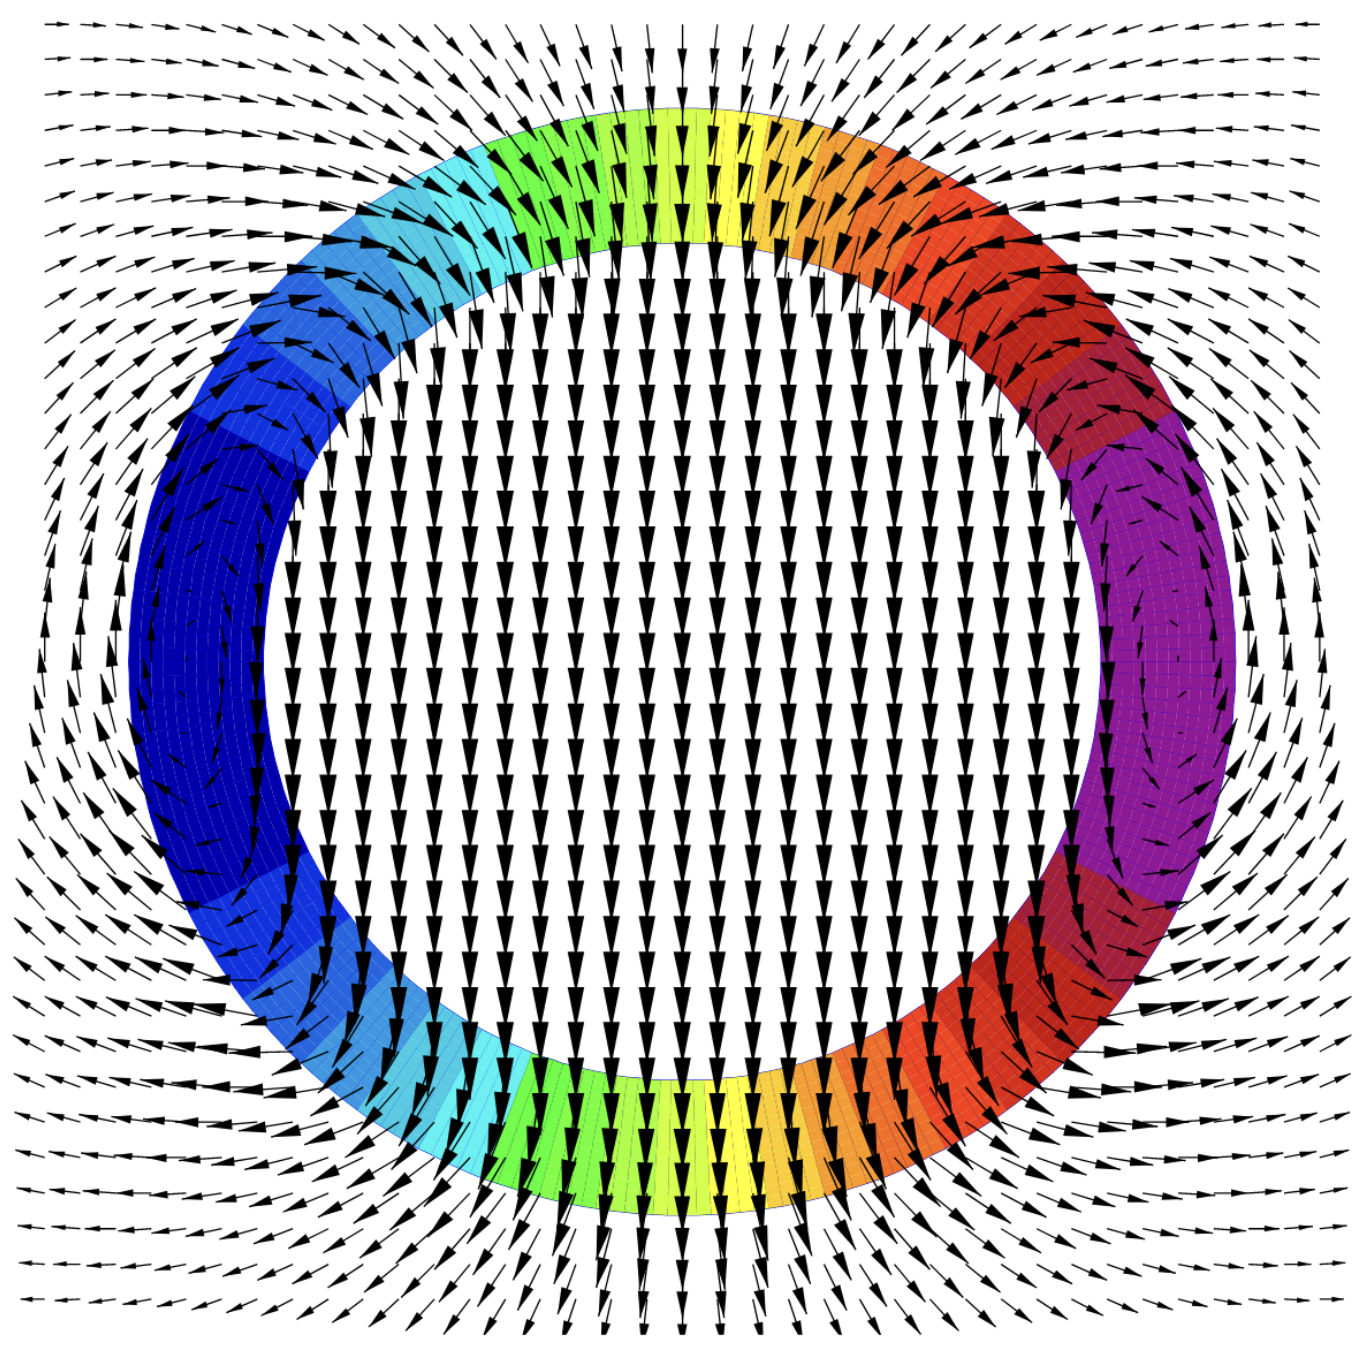
\includegraphics[width=6.5cm]{Figures/Chapter2/ideal_dipole_cos_theta.png}
        \label{fig:ideal_dipole}
    }
    \hspace{0.5cm}
    \subfloat[.8\linewidth][Ideal quadrupole.]{
        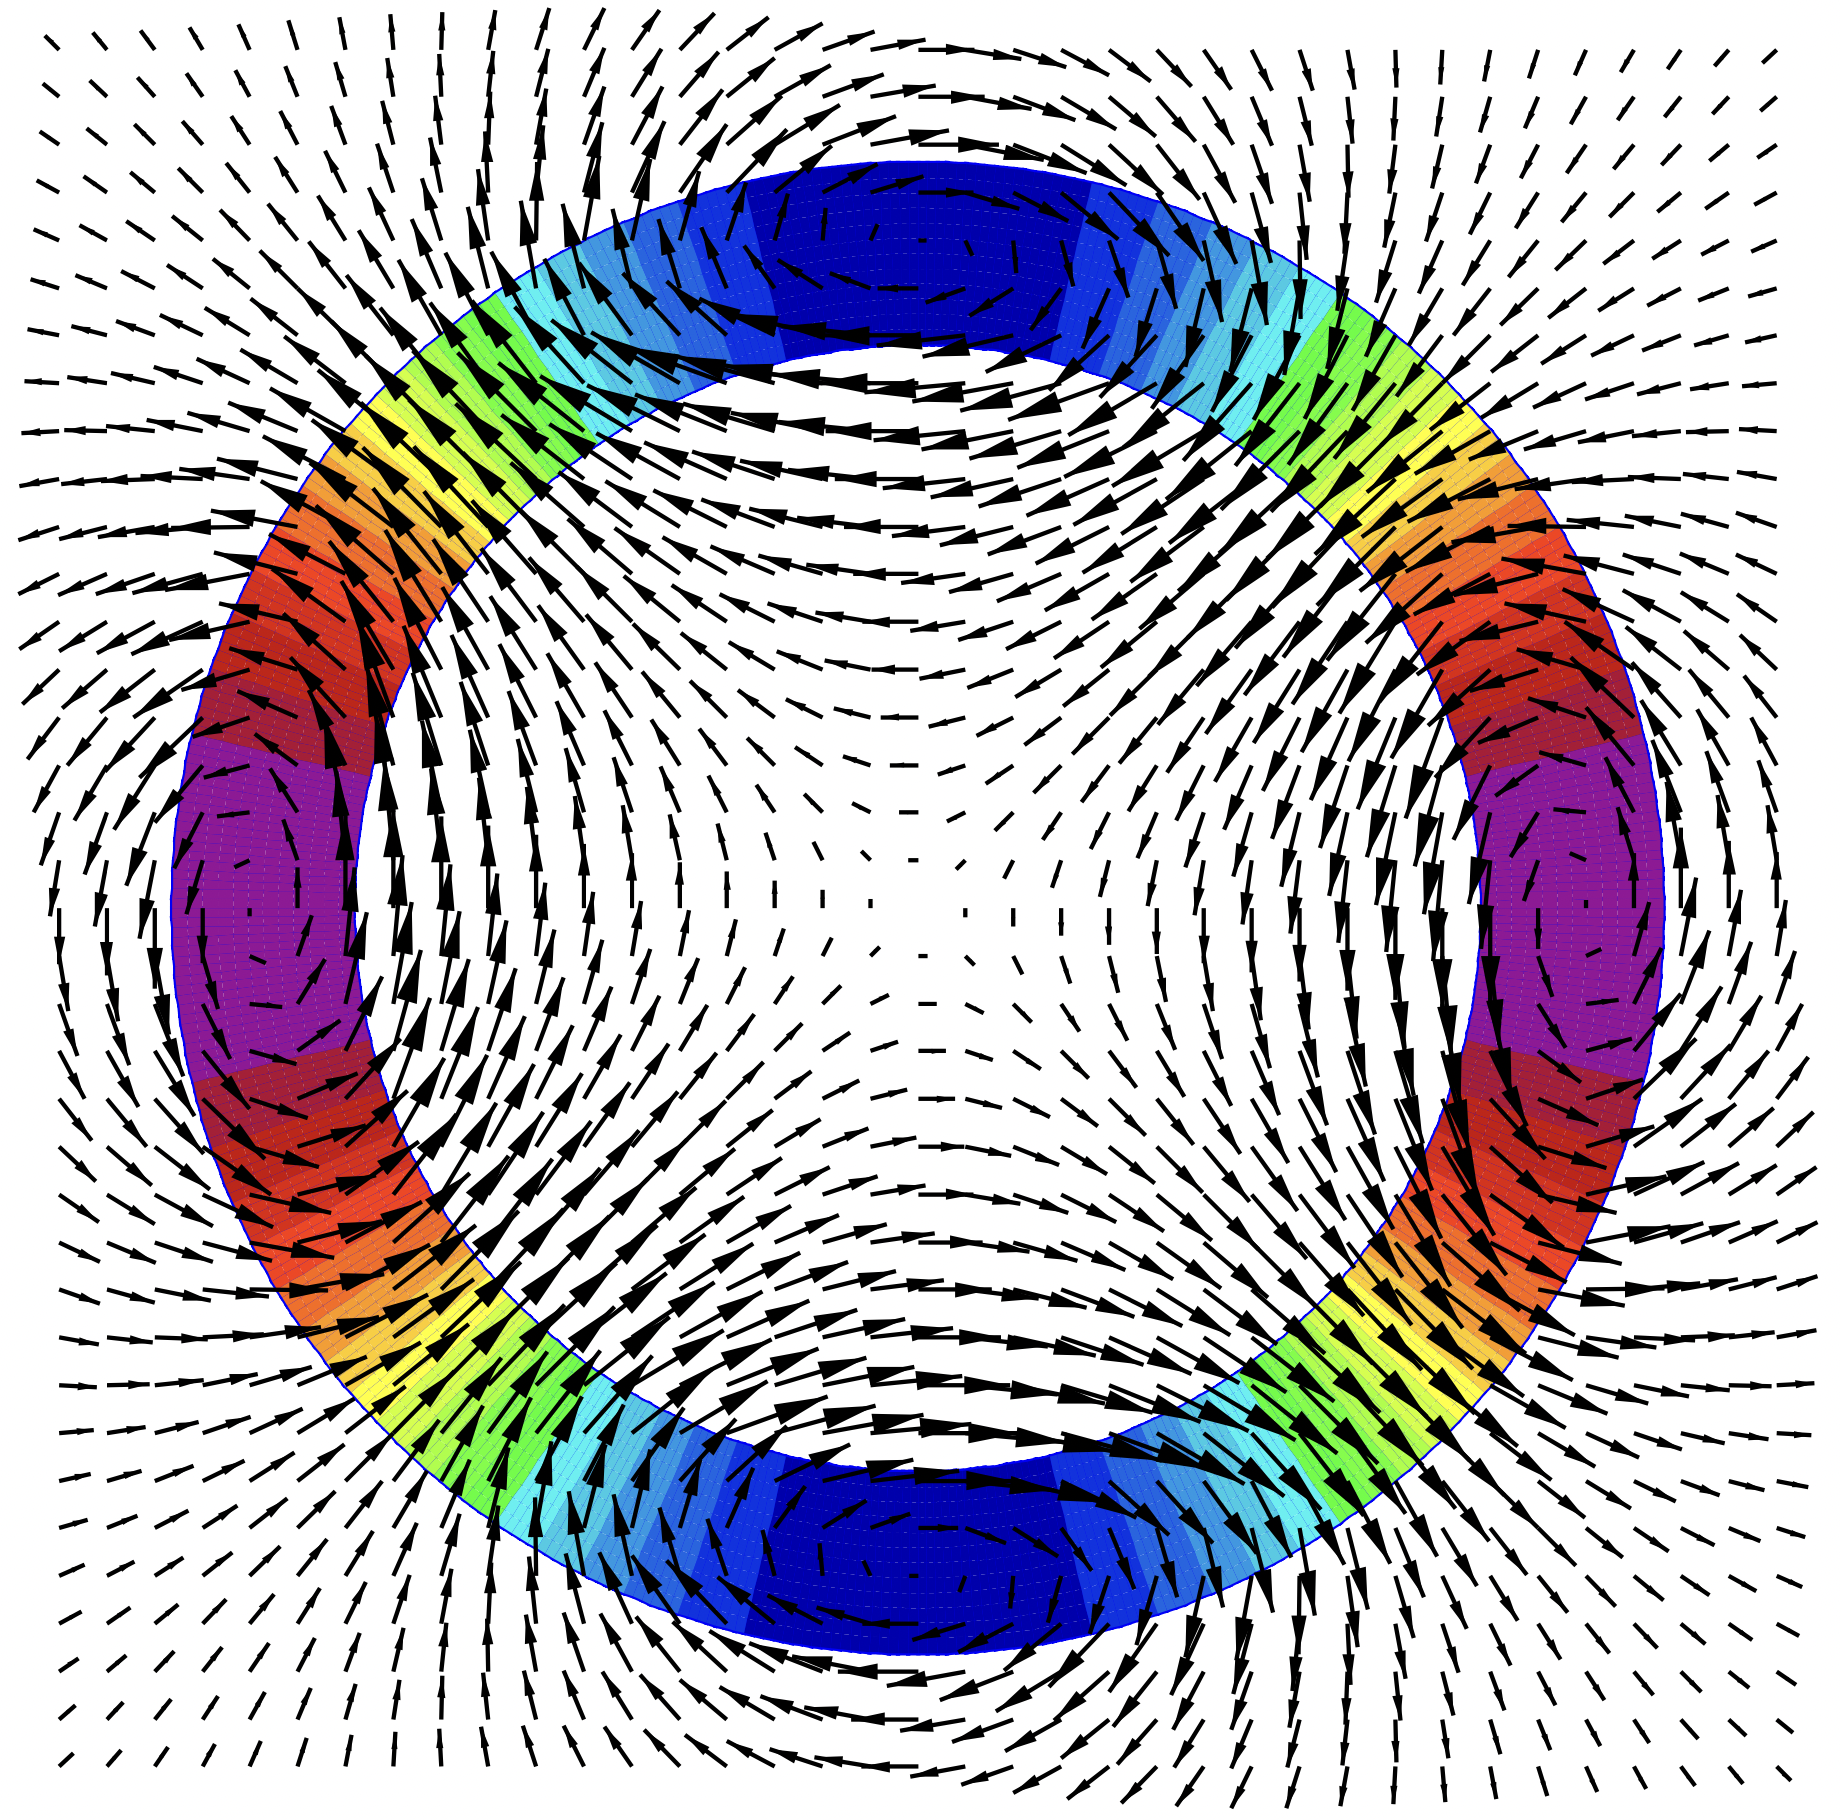
\includegraphics[width=6.5cm]{Figures/Chapter2/ideal_quadrupole_cos_2theta.png}
        \label{fig:ideal_quadrupole}
    }
    \caption{Magnetic fields and forces in an idealized dipole and quadrupole, with a \(\cos(\theta)\) and \(\cos(2\theta)\) current distribution in the circular coil, respectively. Current in the dipole and quadrupole coils are indicated in color. These visuals were taken from \cite{CERN:Russenschuck:CAS_Design_Magnets}.}
    \label{figure:dipole_quadrupole_fields}
\end{figure}

The focusing from quadrupoles in a circular accelerator such as the LHC is periodic in \(s\), with a period of at most the circumference of the machine.
Assuming the existence of a closed orbit, the transverse motion of a single particle in a synchrotron with a periodic lattice is described by Hill's equation:

\begin{equation}
    u^{\prime \prime} + k(s) u = 0; \quad u = x, y; \quad u^{\prime} = \dfrac{du}{ds} ,
    \label{equation:hill_equation}
\end{equation}
where \(k\) describes the focusing forces action on the beam, and varies with \(s\) as it is dictated by magnetic elements traversed by particles.
A focusing quadrupole has a \(k > 0\), a focusing quadrupole has \(k < 0\), and a drift space has \(k = 0\).
According to the theorem of Floquet~\cite{BOOK:Lee:Accelerator_physics}, the solution with periodic boundary conditions to Hill’s equation take the form of \cref{equation:hill_solution}:

\begin{equation}
    \begin{aligned}
        x &= \sqrt{\beta_{x}(s) \varepsilon_{x}} \cos \left(\phi_{x}(s) + \phi_{x_0}\right) \\
        y &= \sqrt{\beta_{y}(s) \varepsilon_{y}} \cos \left(\phi_{y}(s) + \phi_{y_0}\right)
    \end{aligned}
    \label{equation:hill_solution}
\end{equation}

Here \(\beta(s)\) is the \emph{beta-function} and represents the fluctuation of the oscillation envelope around the ring, while \(\varepsilon\) is the \emph{geometric emittance} of a particle and is a constant of the motion at a given energy. 
In particle colliders such as the LHC the \betafunctions at the Interaction Points (IP), where the beams are made to collide, are commonly referred to as \(\beta^{\ast}\).
The difference of the betatron phase functions at two points \(s_1\) and \(s_2\) in the lattice is called the betatron \emph{phase advance} and is defined as:

\begin{equation}
    \mu = \phi(s_{2}) - \phi(s_{1}) = \int_{s_{1}}^{s_{2}} \frac{1}{\beta(s)} ds
\end{equation}

As particles go around the ring, they oscillate around the closed orbit within an enveloppe defined by the \betafunctions and the emittance.
The number of these so-called \emph{betatron oscillations} per revolution is the \emph{tune} \(Q_{x,y}\).
The tune is defined in \cref{equation:tune_definition}, where $\Delta \phi_{x, y}$ is the total betatron \emph{phase advance} of a particle3 over a full circumference:

\begin{equation}
    Q_{x, y} = \frac{1}{2 \pi} \Delta \phi_{x, y} = \frac{1}{2 \pi} \oint_C \dfrac{ds}{\beta_{x, y}(s)}
    \label{equation:tune_definition}
\end{equation}

\todo{Here introduce going through a magnetic element and how we can use a matrix to represent. Do transfer matrix then (Tobias phd, eq 2.3). }

Similarly to the \betafunction, the \emph{gamma-function} $\gamma(s)$ describes the envelope of oscillations in \(x^{\prime}\) and \(y^{\prime}\).
Both quantities are related by the \emph{alpha-function}, defined as:

\begin{equation}
    \alpha_{x, y}(s) = -\frac{1}{2} \dfrac{d}{ds} \beta_{x, y}(s) = \sqrt{\gamma_{x, y}(s) \beta_{x, y}(s) - 1}
    \label{equation:alpha_function}
\end{equation}

In the linear regime all particle trajectories describe ellipses in \((x, x^{\prime})\) and \((y, y^{\prime})\) phase space.
The geometric emittance \(\varepsilon\) introduced in \cref{equation:hill_solution}, also named the \emph{Courant-Snyder invariant}, defines together with the \emph{Twiss parameters} \(\alpha(s)\), \(\beta(s)\) and \(\gamma(s)\) the equation of the phase space ellispe:

\begin{equation}
    \gamma_{u}(s) u^{2} + 2 \alpha_{u}(s) u(s) u^{\prime}(s) + \beta_{u}(s) u^{\prime}(s)^{2} = \varepsilon \quad \text { where } u = x, y
    \label{equation:ellipse_equation}
\end{equation}

\Cref{figure:phase_space_ellipse} shows a schematic illustration of the phase space ellipse, the area of which is defined by the geometric emittance according to:

\begin{equation}
    A = \pi \varepsilon
    \label{equation:phase_space_ellipse_area}
\end{equation}

\begin{figure}[!htb]
    \begin{center}
    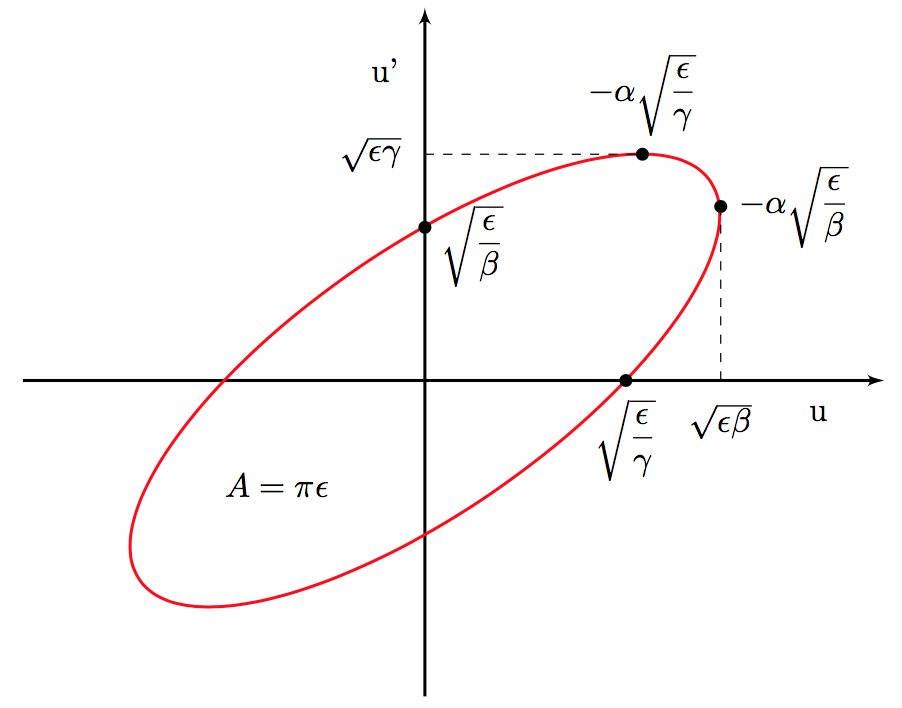
\includegraphics[width = 0.85\linewidth]{Figures/Chapter2/Phase_Space.png}
    \caption{Phase space ellipse in the transverse \((u, u^{\prime})\) plane, where \(u\) represents either transverse coordinate \(x\) or \(y\).}
    \label{figure:phase_space_ellipse}
    \end{center}
\end{figure}

According to the Liouville theorem, the phase space volume, the ellipse area \(A\) is a constant in a closed system.
When accelerating the beam this theorem no longer holds true and the geometric emittance \(\varepsilon\) will decrease as the beam energy increases.
One can then construct the \emph{normalized emittance} \(\varepsilon_{\gamma}\), which is invariant with beam energy, based on the relativistic beta and gamma:

\begin{equation}
    \varepsilon_{\gamma} = (\beta_{\mathrm{rel}} \gamma_{\mathrm{rel}}) \varepsilon
    \label{equation:normalized_emittance}
\end{equation}

When referring to the emittance of a specific particle one uses the term \emph{single particle emittance}.
Different particles in the beam will have different single particle emittances and will undergo betatron oscillations of varying amplitudes.
For a Gaussian shaped beam the particle at a \(1 \sigma\) orbit offset defines the beam size:

\begin{equation}
    \sigma_u = \sqrt{\varepsilon_u \beta_u} \quad \text { where } u = x, y
\end{equation}

Its Courant-Snyder invariant is equivalent with the so-called \emph{beam emittance}, which describes the phase space volume occupied by the particles of the beam, typically taken as the emittance corresponding to a particle amplitude of \(1 \sigma\) in the assumed Gaussian particle distribution.
In the case of more general particle distributions an alternative definition of the beam emittance is often used~\cite{CERN:Muller:Beam_Matter_Covariance_Matrix_Emittance, CERN:Buon:CAS_Beam_Phase_Space_Emittance}:

\begin{equation}
    \epsilon_{rms,u} = \sqrt{\left\langle u \right\rangle^{2} \left\langle u^{\prime} \right\rangle^{2} - \left\langle uu^{\prime} \right\rangle^{2}} \quad \text { where } u = x, y
    \label{equation:beam_emittance}
\end{equation}

The phase space trajectory of a particle depends on the Twiss parameters $\alpha(s)$, $\beta(s)$, and $\gamma(s)$.
One can remove this dependency by performing a coordinate transformation to the \emph{Courant-Snyder coordinates}~\cite{BOOK:Bazzani:Normal_Form_Approach_Betatron_Motion}, defined as:

\begin{equation}
    \left(\begin{array}{c}
    \hat{u} \\
    \hat{u}^{\prime}
    \end{array}\right) = \left(\begin{array}{cc}
    \frac{1}{\sqrt{\beta_{u}(s)}} & \frac{\alpha_{u}(s)}{\sqrt{\beta_{u}(s)}} \\
    0 & \sqrt{\beta_{u}(s)}
    \end{array}\right)\left(\begin{array}{c}
    u \\
    u^{\prime}
    \end{array}\right) \quad \text{ where } u = x, y
    \label{equation:courant_snyder_coordinates}
\end{equation}

where the Courant-Snyder coordinates are denoted by \^{}.
In this new system particles follow circular trajectories in phase space.

Until now, it was assumed that all particles had the intended design momentum \(p_{0}\).
Naturally, in practice particles withing the beam have a distribution in energy and momentum.
For a particle with a momentum \(p \neq p_{0}\) one defines and uses the \textit{relative momentum deviation} \(\delta\): the deviation from the reference orbit from the momentum deviation.

\begin{equation}
    \delta = \frac{\Delta p}{p} = \frac{p - p_{0}}{p_{0}}
    \label{equation:momentum_deviation}
\end{equation}

Such momenta offsets introduce \emph{chromatic errors} in the beam dynamics, for instance \emph{dispersion}.
From the definition of the magnetic rigidity in \cref{equation:magnetic_rigidity}, it follows that particles of different momenta will have different local radii of curvature when going through dipoles, and therefore different 
Different momenta(um?) -> different beam rigidity -> different local radius of curvature in dipoles -> different orbit.

The deviation of an off momentum particle orbit from that of the synchronous particle is defined by the \emph{dispersion function} $D(s)$.
Its contribution to a particle's orbit in a region of non-zero dispersion is described by:

\begin{equation}
    \begin{aligned}
    \Delta x_{\mathrm{dispersion}} &= D_{x}(s) \delta \\
    \Delta y_{\mathrm{dispersion}} &= D_{y}(s) \delta
    \end{aligned}
    \label{equation:dispersion_contribution_to_orbit}
\end{equation}
\bigbreak

The orbit of any given particle is defined by:

\begin{equation}
    u = u_{\mathrm{betatronic}} + u_{\mathrm{dispersion}} + \left.u_{\mathrm{closed \ orbit}} \right\rvert_{\delta = 0} \quad \text{ where } u = x, y
    \label{equation:_particle_orbit}
\end{equation}

%----------------------------------------------------------------------------------------

\section{Non-Linear Magnetic Multipoles}

%----------------------------------------------------------------------------------------

\section{Formalism of Non-Linear Beam Dynamics}

%----------------------------------------------------------------------------------------

\section{Phenomenology of Non-Linear Beam Dynamics}

\subsection{Chromaticity}

\subsection{Detuning with Amplitude}

\subsection{Decoherence}

%----------------------------------------------------------------------------------------

\section{Normal Form Formalism and Resonance Driving Terms}


The derivation in this section follows the approach given in \cite{Tomas_thesis, Franchi_thesis}.
While the non-linear dynamics can not be described with matrices, it can be described by the transfer map formalism.
In the frame where the one turn map is represented by a pure rotation - in normal forms coordinates - it can be written as \cite{Tomas_thesis}:\\

\begin{equation}
    \mathcal{M} = 
    e^{:\eqnmarkbox[blue]{node1}{\tilde{h_{1}}}:}
    e^{:\eqnmarkbox[red]{node2}{\tilde{h_{2}}}:}
    \ldots
    e^{:\eqnmarkbox[green]{noden}{\tilde{h_{n}}}:}
    R
    \label{equation:norm_form_one_turn_map}
\end{equation}
\annotate[yshift=0.5em]{above, left}{node1}{First element}
\annotate[yshift=-0.75em]{below}{node2}{Second element}
\annotate[yshift=0.5em]{above, right}{noden}{Nth element}\\\\
% ------------------ %
where \(e^{:\tilde{h_{1}}:}\) is an exponential Lie operator describing a nonlinear element, and \(\mathbf{R}\) is the rotation matrix describing the linear motion.
This simplifies through the Campbell-Baker-Hausdorff theorem to:

\begin{equation}
    \mathcal{M} = e^{:h:} R
\end{equation}

In case the \(\tilde{h_{n}}\) are small, then \(h\) may be approximated by:

\begin{equation}
    h = \sum_{n=1}^{N} \tilde{h}_{n} + \sum_{n, m<n}^{N} \left[\tilde{h}_{m}, \tilde{h}_{n} \right] + \ldots
    \label{equation:h_expansion}
\end{equation}

Using only the first order in \(\tilde{h_{n}}\), \(h\) may be expanded according to \cref{equation:h_approximation_first_order} using the action-angle variables TODO.

\begin{equation}
    h = \sum_{j k l m} h_{j k l m} \left(2 J_{x}\right)^{\frac{j+k}{2}} \left(2 J_{y}\right)^{\frac{l+m}{2}} e^{i \left[(j-k)\left(\phi_{x}-\phi_{x_{0}}\right) + (l-m)\left(\phi_{y}-\phi_{y_{0}}\right) \right]}
    \label{equation:h_approximation_first_order}
\end{equation}

Here \(h_{j k l m}\) are Hamiltonian coefficients representing the contributions from multipoles of order \(n = j + k + l + m\).
A multipole of order \(n\) generates terms in the Hamiltonian \(\propto x^{j+k} y^{l+m}\), where again \(n = j + k + l + m\).

In the case of a skew quadrupole, such an element gives rise to terms in the Hamiltonian \(\propto xy\), meaning that it contributes to the Hamiltonian terms \(h_{1010}\), \(h_{1001}\), \(h_{0110}\) and \(h_{0101}\).
The idea behind normal form coordinates is to perform a transformation from a system with amplitude and phase dependence to a simpler form.
The simplest form is an amplitude dependent rotation, i.e. a rotation in phase space where the angle depends on the amplitude of the particle.
An excellent approach to normal forms formalism can be found in \cite{Carlier_thesis}.

The coordinate change is represented by a similarity transformation of the one turn map:

\begin{equation}
    e^{-: F:} e^{: h:} R e^{: F:}
\end{equation}
% ------------------ %
where \(F\) is the generating function for the transformation.
The formal solution to finding the generating function F is given in \cite{Forest_normal_forms} and the explicit expression is obtained in \cite{Tomas_thesis} as

\begin{equation}
    F = \sum_{j k l m} f_{j k l m} \left(2 I_{x}\right)^{\frac{j+k}{2}}\left(2 I_{y}\right)^{\frac{l+m}{2}} e^{i\left[(j-k)\left(\psi_{x}-\psi_{x_{0}}\right)+(l-m)\left(\psi_{y}-\psi_{y_{0}}\right)\right]}
    \label{equation:F_generating}
\end{equation}
% ------------------ %
where \(f_{jklm}\) are the resonance driving terms corresponding to the Hamiltonian terms \(h_{jklm}\) respectively.
They can be expressed according to \cref{equation:f_rdts} \cite{Tomas_thesis, Franchi_thesis}, where \(Q_x\) and \(Q_y\) are the unperturbed tunes.

\begin{equation}
    f_{jklm} = \frac{h_{jklm}}{1 - e^{i 2 \pi \left[(j-k) Q_{x} + (l-m) Q_{y} \right]}}
    \label{equation:f_rdts}
\end{equation}
% ------------------ %
\Cref{equation:f_rdts} diverges when \(j, k, l, m, Q_x\) and \(Q_y\) satisfy the condition:

\begin{equation}
    (j-k) Q_{x} + (l-m) Q_{y} = p \quad \text{ where } p \in \mathcal{Z}
    \label{equation:resonance_condition}
\end{equation}
% ------------------ %
Hence, the \(f_{jklm}\) terms are the driving terms of the resonances \([(j-k),(l-m)]\).
Every Hamiltonian term is associated with a resonance, which explains the term Resonance Driving Terms.
The normalized Courant-Snyder coordinates are related to the action-angle variable as

\begin{equation}
    \begin{aligned}
    z &= \sqrt{2 J_{z}} \cos (\phi_{z} - \phi_{z_{0}}) \\
    p_{z} &= -\sqrt{2 J_{z}} \sin (\phi_{z} - \phi_{z_{0}}) \quad \text { where } z=x, y
    \end{aligned}
    \label{equation:courant_snyder_to_action_angle}
\end{equation}
% ------------------ %
It is convenient to introduce the resonant basis h defined as

\begin{equation}
    \begin{aligned}
    h_{z}^{\pm} &= z \pm i p_{z} = \sqrt{2 J_{z}} e^{\mp i \left(\phi_{z}-\phi_{z_{0}}\right)} \quad \text { where } z=x, y \\
    \mathbf{h} &= \left( h_{x}^{+}, h_{x}^{-}, h_{y}^{+}, h_{y}^{-} \right)
    \end{aligned}
    \label{equation:resonant_basis_h}
\end{equation}

The transformation to a new set of Normal Form coordinates \(\left(\zeta_{x}^{+}, \zeta_{x}^{-}, \zeta_{y}^{+}, \zeta_{y}^{-}\right)\) is given by the operator \(e^{: -F :}\).
This is expressed as

\begin{equation}
    \zeta_{z}^{\pm} = \sqrt{2 I_{z}} e^{\pm i \left(\phi_{z}+\phi_{z 0} \right)} = e^{:-F:} h_{z}^{\pm}
    \label{equation:action_angle_to_normal_form}
\end{equation}
% ------------------ %
where \(I_{z}\) is the invariant of motion in the new frame.
The one-turn map in normal form coordinates is by construction an amplitude dependent rotation, and hence the motion in these coordinates as a function of the turn number N is given by

\begin{equation}
    \zeta_{z}^{-}(N) = \sqrt{2 I_{z}} e^{2 \pi \nu_{x} N + \phi z_{0}}
    \label{equation:normal_form_by_turn}
\end{equation}

The inverse transformation from the new action-angle variables to the linearly normalized variable is to first order written as

\begin{equation}
    h_{z}^{-} = e^{: F:} \zeta_{z}^{-} \simeq \zeta_{z}^{-} + \left[F, \zeta_{z}^{-}\right]
    \label{equation:inverse_normal_form_transform}
\end{equation}

and using \cref{equation:normal_form_by_turn} and \cref{equation:inverse_normal_form_transform} the normalized coordinates can be expressed in the form

\begin{equation}
    \begin{aligned}
    h_{x}^{-}(N) &= \sqrt{2 I_{x}} e^{i\left(2 \pi \nu_{x} N - \psi_{x_{0}}\right)} - \\
    & 2 i \sum_{jklm} j f_{jklm} \left(2 I_{x}\right)^{\frac{j+k-1}{2}} \left(2 I_{y}\right)^{\frac{l+m}{2}} e^{i \left[(1-j+k) \left(2 \pi \nu_{x} N-\psi_{x_{0}}\right) + (m-l) \left(2 \pi \nu_{y} N-\psi_{y_{0}}\right) \right]} \\
    h_{y}^{-}(N) &= \sqrt{2 I_{y}} e^{i\left(2 \pi \nu_{y} N - \psi_{y_{0}}\right)} - \\
    & 2 i \sum_{jklm} l f_{jklm} \left(2 I_{x}\right)^{\frac{j+k}{2}} \left(2 I_{y}\right)^{\frac{l+m-1}{2}} e^{i \left[(k-j) \left(2 \pi \nu_{x} N-\psi_{x_{0}}\right) + (1-l+m) \left(2 \pi \nu_{y} N-\psi_{y_{0}}\right) \right]}
    \end{aligned}
    \label{equation:normal_form_coordinates}
\end{equation}

https://cds.cern.ch/record/1533084/files/CERN-THESIS-2013-022.pdf


\section{Betatron Coupling}

Talk about the closest tune approach \(\Delta Q_{\mathrm{min}}\) quantity.
Without betatron coupling in the machine, horizontal and vertical tunes can be matched to the same fractional value.
In the presence of betatron coupling, the \emph{coupled fractional tunes} \(Q_1\) and \(Q_2\) cannot be matched to the same value and a minimal separation can be observed.
This separation is called the \emph{closest tune approach} and is given as the \(\Delta Q_{\mathrm{min}}\) quantity.
\Cref{figure:closest_tune_approach} shows an illustration of the phenomenon, where both the unperturbed and coupled fractional tunes are plotted against the uncoupled tune split.
The closest tune approach is the minimum distance between the two red curves, highlighted by an arrow.

\begin{figure}[!htb]
    \begin{center}
    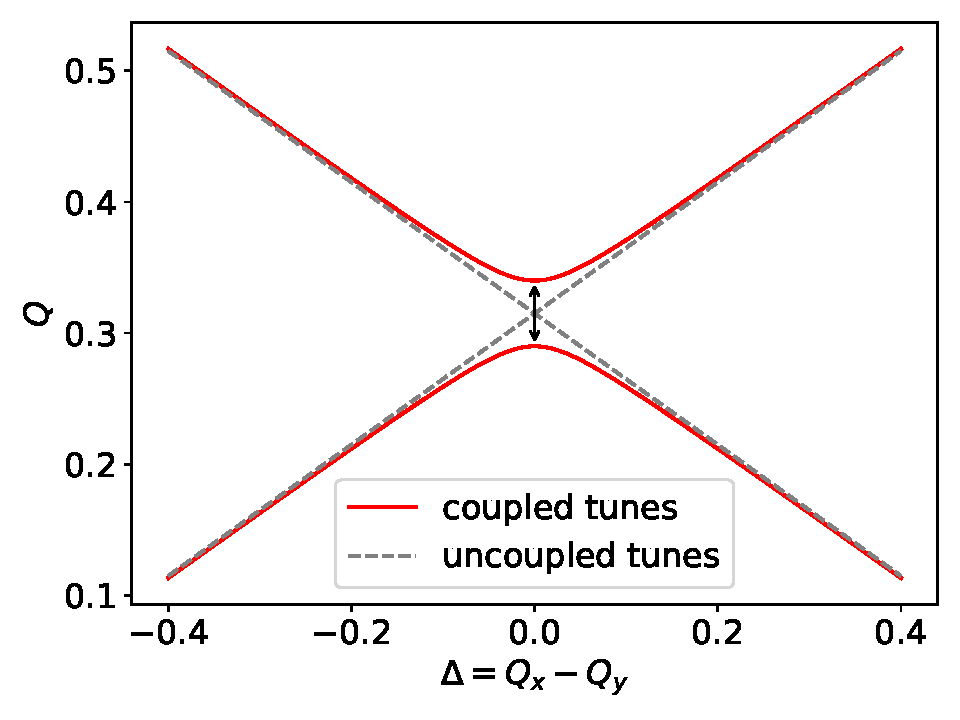
\includegraphics[width = 0.9\linewidth]{Figures/Chapter2/tune_perturbation.pdf}
    \caption{Illustration of coupled and uncoupled fractional tunes versus the uncoupled tune split.}
    \label{figure:closest_tune_approach}
    \end{center}
\end{figure}

%----------------------------------------------------------------------------------------

\section{Luminosity}

%----------------------------------------------------------------------------------------
% Chapter 3

\chapter{Modelling and Correction of the Linear Optics} % Main chapter title

\label{Chapter3} % For referencing the chapter elsewhere, use \ref{Chapter1} 

%----------------------------------------------------------------------------------------

% Define some commands to keep the formatting separated from the content 
%\newcommand{\keyword}[1]{\textbf{#1}}
%\newcommand{\tabhead}[1]{\textbf{#1}}
%\newcommand{\code}[1]{\texttt{#1}}
%\newcommand{\file}[1]{\texttt{\bfseries#1}}
%\newcommand{\option}[1]{\texttt{\itshape#1}}

%----------------------------------------------------------------------------------------

Some paragraph before the first section.

%----------------------------------------------------------------------------------------

\section{Measurement and Correction of the Linear Optics}

\subsection{Linear Optics Measurement}

\subsection{Linear Optics Correction}

%----------------------------------------------------------------------------------------

\section{Comparison of Simulated Linear Optics to Measurement}

%----------------------------------------------------------------------------------------

\section{Commissioning of Linear LHC Optics for Proton Operation at $\beta^{*} = 0.3$m, $6.5$TeV}

\subsection{Injection ($450$GeV)}

\subsection{Top Energy ($6.5$TeV)}

%----------------------------------------------------------------------------------------

\section{Conclusions}

%----------------------------------------------------------------------------------------
% Chapter 4

\chapter{Interaction Region Local Coupling Correction in the LHC} % Main chapter title

\label{Chapter4} % For referencing the chapter elsewhere, use \ref{Chapter1} 

%----------------------------------------------------------------------------------------

% Define some commands to keep the formatting separated from the content 
%\newcommand{\keyword}[1]{\textbf{#1}}
%\newcommand{\tabhead}[1]{\textbf{#1}}
%\newcommand{\code}[1]{\texttt{#1}}
%\newcommand{\file}[1]{\texttt{\bfseries#1}}
%\newcommand{\option}[1]{\texttt{\itshape#1}}

%----------------------------------------------------------------------------------------

Some paragraph before the first section.

%----------------------------------------------------------------------------------------

\section{Linear Coupling in the Interaction Regions}

\subsection{Overview of the IR Layout Difficulties and Why the Phase Advances SUCK}

\subsection{Twiss with Coupling and Ripken parameters}

\subsection{Equivalency of Ripken and Tracking when looking at beam size}

\subsection{Plan for Correction}

%----------------------------------------------------------------------------------------

\section{Measuring Linear Coupling in the Interaction Regions}

\subsection{Relating to outside observables}

%----------------------------------------------------------------------------------------

\section{Proof of principle: Measurement and Correction of Local Coupling in the LHC Interaction Regions}

\subsection{Beam-Based Study of IRs Local Coupling}

\subsection{Simulations of IRs Local Coupling}

%----------------------------------------------------------------------------------------

\section{Impact of Local Coupling Correction on Beam Lifetime}

\subsection{Impact on Tune Footprint}

\subsection{Impact on Dynamic Aperture}

%----------------------------------------------------------------------------------------

\section{Operational Correction Procedure and Run III Commissioning Experience}

\subsection{Procedure}

\subsection{Software}

%----------------------------------------------------------------------------------------

\section{Conclusions}

%----------------------------------------------------------------------------------------
% Chapter 5

\chapter{Experimental Measurement and Correction of Interaction Region Local Coupling in the LHC Run III} % Main chapter title

\label{Chapter5} % For referencing the chapter elsewhere, use \ref{Chapter5}

%----------------------------------------------------------------------------------------

Some paragraph before the first section.

%----------------------------------------------------------------------------------------

\section{Dedicated Measurement and Correction of Local Coupling in IR1 and IR5}

\subsection{Measurement of Local Coupling in the IRs at $\beta^{*}_{IP} = 0.3m$}

\subsection{Correction of Local Coupling in the IRs at $\beta^{*}_{IP} = 0.3m$}

\subsection{Application of Machine Learning for Correction at $\beta^{*}_{IP} = 0.3m$}

%----------------------------------------------------------------------------------------

\section{LHC Run III Commissioning Experience}

%----------------------------------------------------------------------------------------

\section{Conclusions}

%----------------------------------------------------------------------------------------
\chapter{Experimental Measurement and Correction of Interaction Region Local Coupling in the LHC Run III} % Main chapter title

\label{Chapter:Experimental_Results} % For referencing the chapter elsewhere, use \cref{Chapter:Experimental_Results}

%----------------------------------------------------------------------------------------

Some paragraph before the first section.

%----------------------------------------------------------------------------------------

\section{Beam Tests 2021 Results}

Can refer to appendix \Cref{AppendixB} for the fills used.

\section{Measurement and Correction of Local Coupling in the IRs at $\beta^{*}_{IP} = 0.3m$}

Can refer to appendix \Cref{AppendixB} for the fills used.

%----------------------------------------------------------------------------------------

\section{2022 LHC MD Blocks Results (Containment Plans)}

%----------------------------------------------------------------------------------------

\section{Conclusions}

%----------------------------------------------------------------------------------------
% Summary

\chapter{Conclusions}
% \addcontentsline{toc}{chapter}{Conclusions}  % if not numbered chapter

\label{Conclusion} % For referencing the chapter elsewhere, use \Cref{Conclusion}

%----------------------------------------------------------------------------------------

Food for thought here:
\begin{enumerate}
    \item 
\end{enumerate}

%----------------------------------------------------------------------------------------



%----------------------------------------------------------------------------------------
%	BIBLIOGRAPHY
%----------------------------------------------------------------------------------------

\printbibliography
\addcontentsline{toc}{chapter}{Bibliography}

%----------------------------------------------------------------------------------------
%	THESIS CONTENT - APPENDICES
%----------------------------------------------------------------------------------------

\appendix % Cue to tell LaTeX that the following "chapters" are Appendices

% Appendix A
\chapter{Element Naming Conventions in the LHC} % Main appendix title

\label{Appendix_Naming_Conventions} % For referencing this appendix elsewhere, use \Cref{AppendixA}

%----------------------------------------------------------------------------------------

As element names occur often in this document, it is worth spending an appendix detailing the element naming convention in the LHC and HL-LHC.
\Cref{figure:lhc_segment_naming_scheme} below shows the established scheme for a segment of the LHC.

\begin{figure}[h]
    \centering
    \includegraphics*[width=0.9\linewidth]{Figures/Appendices/LHC_naming_scheme.pdf}
    \caption{In-depth view of the naming scheme in a segment of the LHC.}
    \label{figure:lhc_segment_naming_scheme}
  \end{figure}

The general structure goes as follows:
\begin{enumerate}
    \item Each octant is divided into two \textit{half-arcs} surrounding an \textit{insertion}.
    \item Each octant is divided into a left side and a right side.
    \item The center point of some octants is the \textit{Interaction Point} or $\mathrm{IP}$, with their surroundiing region sometimes also referred to as \textit{Interaction Region} ($\mathrm{IR}$).
\end{enumerate}

From the perspective of lattice definitions, there are eight $\mathrm{IP}$s, but this is only for notational ease.
An interaction point in the strict sense is a point where the two beams collide, which is only a feature of octant 1, 2, 5 and 8 where experiments are run.
When an $\mathrm{IP}$ or $\mathrm{IR}$ is referred to in this document, it is taken for granted that it applies to one of these octants.
What all octants nevertheless have in common is that they all have a long straight section in the middle as part of the insertion.
The arc can be perceived to be roughly uniform across LHC whereas the long sections differ from octant to octant.


As the base pattern is a FODO lattice, the machine can be broken up into half-cells containing one quadrupole each.
In doing so, each half-cell is given a number, where the $i^{th}$ quadrupole away from the center of its octant is associated with the $i^{th}$ half-cell.
With this in mind, the general naming convention can be summarized as follows:

% TODO: fix this!
% \begin{align*}
%     \label{eq:lhc_naming_nomenclature}
%     $<TYPE><SPECIAL>.<EXTRA><HALF_CELL><LR><OCTANT>.B<12>$
% \end{align*}

\begin{itemize}
    \item $\mathrm{TYPE}$: Entry specifying the type of element. See \cref{table:element_prefix_examples} for examples.
    \item $\mathrm{SPECIAL}$: Optional entry which can be used to sub-type an element, e.g. $\mathrm{H}$ or $\mathrm{V}$ to signify if a corrector is acting on the horizontal or vertical plane.
    \item $\mathrm{EXTRA}$: Optional entry used to separate between otherwise identically named elements. E.g. $\mathrm{A}$, $\mathrm{B}$, $\mathrm{C}$ to separate between three bending magnets in the same half-cell
    \item $\mathrm{LR}$: Entry specifying which side of the closest $\mathrm{IP}$ the element is on. Assumes either $\mathrm{L}$ (\textit{left}) or $\mathrm{R}$ (\textit{right}).
    \item $\mathrm{OCTANT}$: Entry specifying the octant the element is a part of. Valid entries are integers from $1$ to $8$.
    \item $\mathrm{12}$: Entry specifying which beam the element is part of. Either $1$ or $2$, unless the element is shared between the two beams in which case the element name ends with the $\mathrm{OCTANT}$ entry.
\end{itemize}

\begin{table}[!hbt]
    \centering
    \begin{tabular}{|c|c|}
        \toprule
        \textbf{Element Type} & \textbf{Prefix}   \\
        \midrule
            Bending Magnet    & $\mathrm{MB}$       \\
            Quadrupole        & $\mathrm{MQ}$       \\
            Orbit  Corrector  & $\mathrm{MCB}$      \\
            BPM               & $\mathrm{BPM}$      \\
            Crab Cavity       & $\mathrm{ACFCA}$    \\
            Drift             & $\mathrm{DRIFT}$    \\
        \bottomrule
    \end{tabular}
    \caption{Example prefixes for different LHC element types.}
    \label{table:element_prefix_examples}
 \end{table}

For instance, the element $\mathrm{MQ.25L5.B1}$ is a quadrupole on the left side of $\mathrm{IP5}$, in the $25^{th}$ half-cell and for beam $1$.
The special identifier can be used in multiple ways, for example $\mathrm{MQML.10R1.B1}$ is a different type of quadrupole in half-cell $10$, on the right side of $\mathrm{IP1}$ for beam $1$.
Here the special identifier describes the type of quadrupole.
For $\mathrm{MCBH.21R5.B1}$, the special identifier $\mathrm{H}$ signifies that it is a horizontal orbit corrector.
In the triplet quadrupoles one can notice for instance elements $\mathrm{MQXB.A2L1}$ and $\mathrm{MQXB.B2L1}$.
In this case the elements share type $\mathrm{MQXB}$ (middle, single aperture inner triplet quadrupole), octant, side of $\mathrm{IP}$ and half-cell, which is why they make use of the extra specifiers $\mathrm{A}$ and $\mathrm{B}$ to tell them apart.

Note that these elements skip the appendage of $\mathrm{.B<12>}$.
These correspond to elements common to both beams, which can only happen in the $\mathrm{IR}$.
This is due to the fact that when two beams are brought to collision they pass through the same equipment close to the point of collision.

% Full details can be found in: https://edms.cern.ch/ui/file/103369/3.2/LHC-PM-QA-204-32-00.pdf,  https://edms.cern.ch/ui/#!master/navigator/document?D:1929919921:1929919921:subDocs.
% Appendix B
\chapter{Experimental Knobs Designed for the LHC} % Main appendix title

\label{AppendixB} % For referencing this appendix elsewhere, use \Cref{AppendixB}

One can find in this Appendix the full information of the different experimental knobs that were designed for the LHC.
The knobs are reported below as they have been implemented in the LHC Software Architecture (LSA) framework.
In each case, the values correspond to a trim factor of the knob of \num{1}, and scale linearly with the trim factor.

These knobs have been designed for all beam processes of the LHC Run~3 optics as they were at the time of the 2022 commissioning, for a beam energy of \qty{6800}{\giga\electronvolt}.

%----------------------------------------------------------------------------------------

\section{Definitions of the Colinearity Knobs}

\Cref{table:lsa_ip1_colinearity_knob,table:lsa_ip5_colinearity_knob} show the settings used in LSA to define the colinearity knobs at \(\mathrm{IR1}\) and \(\mathrm{IR5}\).
These knobs control the skew quadrupole correctors left and right of the \IP, the \(\mathrm{MQSX}\) magnets.

\begin{table}[!hbt]
    \centering
    \caption{Definition of the colinearity knob for IR1 as implemented in LSA.}
    \begin{tblr}{colspec={cc}}
        \hline
        \textbf{Component} & \textbf{Value} \\
        \hline
        $\mathrm{RQSX3.L1/K1S}$  &  \num{1E-4}  \\
        $\mathrm{RQSX3.R1/K1S}$  &  \num{-1E-4}  \\
        \hline
     \end{tblr}
    \label{table:lsa_ip1_colinearity_knob}
\end{table}

\begin{table}[!hbt]
    \centering
    \caption{Definition of the colinearity knob for IR5 as implemented in LSA.}
    \begin{tblr}{colspec={cc}}
        \hline
        \textbf{Component} & \textbf{Value} \\
        \hline
        $\mathrm{RQSX3.L5/K1S}$  &  \num{1E-4}  \\
        $\mathrm{RQSX3.R5/K1S}$  &  \num{-1E-4}  \\
        \hline
     \end{tblr}
    \label{table:lsa_ip5_colinearity_knob}
\end{table}

%----------------------------------------------------------------------------------------

\section{Definitions of the Rigid Waist Shift Knobs}

\Cref{table:lsa_ip1_rigid_waist_shift,table:lsa_ip5_rigid_waist_shift} show the settings used in LSA to define the rigid waist shift knobs at \(\mathrm{IR1}\) and \(\mathrm{IR5}\).
These knobs control the triplet magnets left and right of the \IP in order to move all four betatron waists simultaneously.

\begin{table}[!hbt]
    \centering
    \caption{Definition of the rigid waist shift knob for IR1 as implemented in LSA.}
    \begin{tblr}{colspec={cc}}
        \hline
        \textbf{Component} & \textbf{Value} \\
        \hline
        $\mathrm{MQXA1.L1/K1}$  &  \num{-4.38891E-5}  \\
        $\mathrm{MQXA1.R1/K1}$  &  \num{-4.38891E-5}  \\
        $\mathrm{MQXA3.L1/K1}$  &  \num{-4.38891E-5}  \\
        $\mathrm{MQXA3.R1/K1}$  &  \num{-4.38891E-5}  \\
        $\mathrm{MQXB2.L1/K1}$  &  \num{4.38891E-5}  \\
        $\mathrm{MQXB2.R1/K1}$  &  \num{4.38891E-5}  \\
        \hline
     \end{tblr}
    \label{table:lsa_ip1_rigid_waist_shift}
\end{table}

\begin{table}[!hbt]
    \centering
    \caption{Definition of the rigid waist shift knob for IR5 as implemented in LSA.}
    \begin{tblr}{colspec={cc}}
        \hline
        \textbf{Component} & \textbf{Value} \\
        \hline
        $\mathrm{MQXA1.L5/K1}$  &  \num{-4.38891E-5}  \\
        $\mathrm{MQXA1.R5/K1}$  &  \num{-4.38891E-5}  \\
        $\mathrm{MQXA3.L5/K1}$  &  \num{-4.38891E-5}  \\
        $\mathrm{MQXA3.R5/K1}$  &  \num{-4.38891E-5}  \\
        $\mathrm{MQXB2.L5/K1}$  &  \num{4.38891E-5}  \\
        $\mathrm{MQXB2.R5/K1}$  &  \num{4.38891E-5}  \\
        \hline
     \end{tblr}
    \label{table:lsa_ip5_rigid_waist_shift}
\end{table}

%----------------------------------------------------------------------------------------

\section{Definitions of the Optics Rematching Knobs}

\Cref{table:lsa_ip1_pos_rematching_knob,table:lsa_ip1_neg_rematching_knob} show the settings used in LSA to define the optics rematching knobs needed after applying the rigid waist shift knob, at \(\mathrm{IR1}\).
\Cref{table:lsa_ip1_pos_rematching_knob} gives the settings that rematch the optics when the \(\mathrm{IR1}\) rigid waist shift knob is applied with a factor of \num{1}, while \cref{table:lsa_ip1_neg_rematching_knob} gives the settings that rematch the optics when the \(\mathrm{IR1}\) rigid waist shift knob is applied with a factor of \num{-1}.
These knobs control the independent magnets \(\mathrm{Q4}\) to \(\mathrm{Q10}\) left and right of the \IP for both beams.

\begin{table}[!hbt]
    \centering
    \caption{Definition of the optics rematching knob for \(\mathrm{IR1}\) as implemented in LSA. These settings rematch the optics for an applied rigid waist shift knob trimmed with a factor \num{1}.}
    \begin{tblr}{colspec={ccc}}
        \hline
        \textbf{Component} & \textbf{Beam 1 Value} & \textbf{Beam 2 Value} \\
        \hline
        $\mathrm{RQ4.L1B[12]/K1}$   &  \num{7.35134890419431E-5}    &  \num{3.132269910111063E-7}   \\
        $\mathrm{RQ4.R1B[12]/K1}$   &  \num{4.7040823119459674E-5}  &  \num{5.434962804429233E-5}   \\
        $\mathrm{RQ5.L1B[12]/K1}$   &  \num{-2.1422146528493613E-4} &  \num{1.2834816880058497E-4}  \\
        $\mathrm{RQ5.R1B[12]/K1}$   &  \num{-2.0866523846052587E-4} &  \num{-1.782987965270877E-5}  \\
        $\mathrm{RQ6.L1B[12]/K1}$   &  \num{1.2522698671091348E-4}  &  \num{-6.654750904999673E-5}  \\
        $\mathrm{RQ6.R1B[12]/K1}$   &  \num{2.1812783961649984E-4}  &  \num{4.843161514145322E-5}   \\
        $\mathrm{RQ7.L1B[12]/K1}$   &  \num{-1.6543477613595314E-5} &  \num{-6.727209893142572E-6}  \\
        $\mathrm{RQ7.R1B[12]/K1}$   &  \num{-2.380601472395938E-5}  &  \num{7.671464118175209E-5}   \\
        $\mathrm{RQ8.L1B[12]/K1}$   &  \num{4.701971556642093E-5}   &  \num{-7.422834642056841E-6}  \\
        $\mathrm{RQ8.R1B[12]/K1}$   &  \num{-5.1663089834619313E-5} &  \num{2.816191772581078E-5}   \\
        $\mathrm{RQ9.L1B[12]/K1}$   &  \num{1.1833090684376657E-4}  &  \num{-1.835947623476386E-4}  \\
        $\mathrm{RQ9.R1B[12]/K1}$   &  \num{1.3951913570053875E-4}  &  \num{-6.844480230938643E-5}  \\
        $\mathrm{RQ10.L1B[12]/K1}$  &  \num{-2.4705037503736094E-5} &  \num{-1.4153616211842746E-4} \\
        $\mathrm{RQ10.R1B[12]/K1}$  &  \num{-1.960854024218861E-5}  &  \num{-1.2572514242492616E-4} \\
        \hline
     \end{tblr}
    \label{table:lsa_ip1_pos_rematching_knob}
\end{table}

\begin{table}[!hbt]
    \centering
    \caption{Definition of the optics rematching knob for \(\mathrm{IR1}\) as implemented in LSA. These settings rematch the optics for an applied rigid waist shift knob trimmed with a factor \num{-1}.}
    \begin{tblr}{colspec={ccc}}
        \hline
        \textbf{Component} & \textbf{Beam 1 Value} & \textbf{Beam 2 Value} \\
        \hline
        $\mathrm{RQ4.L1B[12]/K1}$   &  \num{2.890068935812451E-5}   &  \num{5.81979111302644E-5}    \\
        $\mathrm{RQ4.R1B[12]/K1}$   &  \num{-3.1025800126371905E-5} &  \num{1.7403455785824917E-5}  \\
        $\mathrm{RQ5.L1B[12]/K1}$   &  \num{1.7946695152204484E-5}  &  \num{-2.591577358543873E-4}  \\
        $\mathrm{RQ5.R1B[12]/K1}$   &  \num{2.076919045066461E-4}   &  \num{-5.6730073993094265E-5} \\
        $\mathrm{RQ6.L1B[12]/K1}$   &  \num{4.143969636061229E-5}   &  \num{3.008508065249771E-4}     \\
        $\mathrm{RQ6.R1B[12]/K1}$   &  \num{-1.848040847107768E-4}  &  \num{-6.006251715007238 E-5} \\
        $\mathrm{RQ7.L1B[12]/K1}$   &  \num{5.634562694467604E-5}   &  \num{-3.647266566986218E-5}  \\
        $\mathrm{RQ7.R1B[12]/K1}$   &  \num{-8.4415096353041E-6}    &  \num{5.911061293772946E-7}   \\
        $\mathrm{RQ8.L1B[12]/K1}$   &  \num{3.5822893551085144E-5}  &  \num{-1.7834593018051237E-4} \\
        $\mathrm{RQ8.R1B[12]/K1}$   &  \num{1.4469090092461556E-4}  &  \num{1.1235206329729408E-4}  \\
        $\mathrm{RQ9.L1B[12]/K1}$   &  \num{-1.0561864473856986E-4} &  \num{6.79645236232318E-5}    \\
        $\mathrm{RQ9.R1B[12]/K1}$   &  \num{-1.68628481333144E-4}   &  \num{1.1431280290707946E-4}  \\
        $\mathrm{RQ10.L1B[12]/K1}$  &  \num{-8.416329364990816E-5}  &  \num{-1.8715139958658256E-5} \\
        $\mathrm{RQ10.R1B[12]/K1}$  &  \num{-4.208946484141052E-5}  &  \num{4.75086308142636E-5}    \\
        \hline
     \end{tblr}
    \label{table:lsa_ip1_neg_rematching_knob}
\end{table}


\Cref{table:lsa_ip5_pos_rematching_knob,table:lsa_ip5_neg_rematching_knob} show the settings used in LSA to define the optics rematching knobs needed after applying the rigid waist shift knob, at \(\mathrm{IR5}\).
\Cref{table:lsa_ip5_pos_rematching_knob} gives the settings that rematch the optics when the \(\mathrm{IR5}\) rigid waist shift knob is applied with a factor of \num{1}, while \cref{table:lsa_ip1_neg_rematching_knob} gives the settings that rematch the optics when the \(\mathrm{IR5}\) rigid waist shift knob is applied with a factor of \num{-1}.
These knobs control the independent magnets \(\mathrm{Q4}\) to \(\mathrm{Q10}\) left and right of the \IP for both beams.

\begin{table}[!hbt]
    \centering
    \caption{Definition of the optics rematching knob for \(\mathrm{IR5}\) as implemented in LSA. These settings rematch the optics for an applied rigid waist shift knob trimmed with a factor \num{1}.}
    \begin{tblr}{colspec={ccc}}
        \hline
        \textbf{Component} & \textbf{Beam 1 Value} & \textbf{Beam 2 Value} \\
        \hline
        $\mathrm{RQ4.L5B[12]/K1}$   &  \num{4.732644447358325E-5}   &  \num{7.708167117925768E-7}   \\
        $\mathrm{RQ4.R5B[12]/K1}$   &  \num{2.995622344315052E-5}   &  \num{5.22927766724024E-5}    \\
        $\mathrm{RQ5.L5B[12]/K1}$   &  \num{-1.5405772137455642E-4} &  \num{1.3209861936047673E-4}  \\
        $\mathrm{RQ5.R5B[12]/K1}$   &  \num{-1.541586680104956E-4}  &  \num{-2.5072691641980782E-5} \\
        $\mathrm{RQ6.L5B[12]/K1}$   &  \num{8.088711911113933E-5}   &  \num{-7.675093365833163E-5}  \\
        $\mathrm{RQ6.R5B[12]/K1}$   &  \num{9.079173469217494E-5}   &  \num{8.68605129653588E-5}    \\
        $\mathrm{RQ7.L5B[12]/K1}$   &  \num{-5.050462277722545E-5}  &  \num{6.267658591241343E-6}   \\
        $\mathrm{RQ7.R5B[12]/K1}$   &  \num{-2.046442386927083E-5}  &  \num{7.702426955802366E-5}   \\
        $\mathrm{RQ8.L5B[12]/K1}$   &  \num{8.284445357276127E-5}   &  \num{1.469226845074445E-5}   \\
        $\mathrm{RQ8.R5B[12]/K1}$   &  \num{-1.498689925938379E-5}  &  \num{6.506405043182895E-5}   \\
        $\mathrm{RQ9.L5B[12]/K1}$   &  \num{1.33068417198956E-4}    &  \num{-1.746977650327608E-4}  \\
        $\mathrm{RQ9.R5B[12]/K1}$   &  \num{1.770079106790945E-4}   &  \num{-7.499273488065228E-5}  \\
        $\mathrm{RQ10.L5B[12]/K1}$  &  \num{3.7454233279277105E-6}  &  \num{-1.4056455984245986E-4} \\
        $\mathrm{RQ10.R5B[12]/K1}$  &  \num{3.122093403362669E-5}   &  \num{-1.1992135841865093E-4} \\
        \hline
     \end{tblr}
    \label{table:lsa_ip5_pos_rematching_knob}
\end{table}

\begin{table}[!hbt]
    \centering
    \caption{Definition of the optics rematching knob for \(\mathrm{IR5}\) as implemented in LSA. These settings rematch the optics for an applied rigid waist shift knob trimmed with a factor \num{-1}.}
    \begin{tblr}{colspec={ccc}}
        \hline
        \textbf{Component} & \textbf{Beam 1 Value} & \textbf{Beam 2 Value} \\
        \hline
        $\mathrm{RQ4.L5B[12]/K1}$   &  \num{3.2619271223666146E-5}  &  \num{6.39320132904686E-5}    \\
        $\mathrm{RQ4.R5B[12]/K1}$   &  \num{-3.05984758597333E-5}   &  \num{2.0575140297296457E-5}  \\
        $\mathrm{RQ5.L5B[12]/K1}$   &  \num{1.5781564798089676E-5}  &  \num{-2.813483588397503E-4}  \\
        $\mathrm{RQ5.R5B[12]/K1}$   &  \num{2.063856809400022E-4}   &  \num{-5.432443867903203E-5}  \\
        $\mathrm{RQ6.L5B[12]/K1}$   &  \num{2.6180659915553406E-5}  &  \num{3.291553002782166E-4}   \\
        $\mathrm{RQ6.R5B[12]/K1}$   &  \num{-1.6515587049070746E-4} &  \num{-7.698741683270782E-5}  \\
        $\mathrm{RQ7.L5B[12]/K1}$   &  \num{6.2934348534327E-5}     &  \num{-4.279221684555523E-5}  \\
        $\mathrm{RQ7.R5B[12]/K1}$   &  \num{-1.3081962606520392E-5} &  \num{1.0687855137803126E-5}  \\
        $\mathrm{RQ8.L5B[12]/K1}$   &  \num{1.700830580375623E-5}   &  \num{-2.078329853247851E-4}  \\
        $\mathrm{RQ8.R5B[12]/K1}$   &  \num{1.206262968480587E-4}   &  \num{1.1532680946402252E-4}  \\
        $\mathrm{RQ9.L5B[12]/K1}$   &  \num{-9.63377024163492E-5}   &  \num{4.971278031007387E-5}   \\
        $\mathrm{RQ9.R5B[12]/K1}$   &  \num{-1.70511455507949E-4}   &  \num{1.1992931104032323E-4}  \\
        $\mathrm{RQ10.L5B[12]/K1}$  &  \num{-8.92050375114195E-5}   &  \num{-1.3822291293763556E-5} \\
        $\mathrm{RQ10.R5B[12]/K1}$  &  \num{-6.2934348534327E-5}    &  \num{4.006792005384341E-5}   \\
        \hline
     \end{tblr}
    \label{table:lsa_ip5_neg_rematching_knob}
\end{table}

% Appendix C
\chapter{List of LHC Fills Used for Measurements} % Main appendix title

\label{AppendixC} % For referencing this appendix elsewhere, use \Cref{AppendixB}

One can find in this Appendix the fully detailed list of LHC fills considered for the experimental campaign.


%----------------------------------------------------------------------------------------

\section{Fills Used During the 2021 Beam Tests}

One can find in this Appendix the fully detailed list of LHC fills considered for the experimental campaign.
\Cref{table:beam_test_fills} reports this list together with the dates, energies, the reason for the following beam dump and some eventual comments.

\begin{table}[!hbt]
    \centering
    \caption{List of the LHC fills used in the experimental campaign, during the LHC Run~\num{3} Commissioning.}
    \begin{tblr}{colspec={ccccc}}
        \hline
        \textbf{Fill \#} & \textbf{Date} & \textbf{Energy [\unit[detect-all]{\giga\electronvolt}]} & \textbf{Dump} & \textbf{Comments}  \\
        \hline
        6000  &  15/04/2022  &  450  &  Normal  &  None  \\
        6000  &  15/04/2022  &  450  &  Normal  &  None  \\
        6000  &  15/04/2022  &  450  &  Normal  &  None  \\
        \hline
     \end{tblr}
    \label{table:beam_test_fills}
 \end{table}

 \section{Fills Used During the LHC Run III Commissioning}

One can find in this Appendix the fully detailed list of LHC fills considered for the experimental campaign.
\Cref{table:run3_fills} reports this list together with the dates, energies, the reason for the following beam dump and some eventual comments.

\begin{table}[!hbt]
    \centering
    \caption{List of the LHC fills used in the experimental campaign, during the LHC Run~\num{3} Commissioning.}
    \begin{tblr}{colspec={ccccc}}
        \hline
        \textbf{Fill \#} & \textbf{Date} & \textbf{Energy [\unit[detect-all]{\giga\electronvolt}]} & \textbf{Dump} & \textbf{Comments}  \\
        \hline
        6000  &  15/04/2022  &  450  &  Normal  &  None  \\
        6000  &  15/04/2022  &  450  &  Normal  &  None  \\
        6000  &  15/04/2022  &  450  &  Normal  &  None  \\
        \hline
     \end{tblr}
    \label{table:run3_fills}
 \end{table}


 \section{Fills Used During the LHC Run III MD Blocks}

 One can find in this Appendix the fully detailed list of LHC fills considered for the experimental campaign.
\Cref{table:md_fills} reports this list together with the dates, energies, the reason for the following beam dump and some eventual comments. 
 
\begin{table}[!hbt]
    \centering
    \caption{List of the LHC fills used in the experimental campaign, during the LHC Run~\num{3} Commissioning.}
    \begin{tblr}{colspec={ccccc}}
        \hline
        \textbf{Fill \#} & \textbf{Date} & \textbf{Energy [\unit[detect-all]{\giga\electronvolt}]} & \textbf{Dump} & \textbf{Comments}  \\
        \hline
        6000  &  15/04/2022  &  450  &  Normal  &  None  \\
        6000  &  15/04/2022  &  450  &  Normal  &  None  \\
        6000  &  15/04/2022  &  450  &  Normal  &  None  \\
        \hline
     \end{tblr}
    \label{table:md_fills}
 \end{table}

% Appendix D

\chapter{Comparison of Different Predictive Machine Learning Models} % Main appendix title

\label{AppendixD} % For referencing this appendix elsewhere, use \Cref{AppendixB}

%----------------------------------------------------------------------------------------

Some content.

\section{Models for the Prediction of Betatron Coupling Sources}

\section{Models for the Prediction of Correction Settings}

%----------------------------------------------------------------------------------------

\end{document}